% This is LLNCS.DEM the demonstration file of
% the LaTeX macro package from Springer-Verlag
% for Lecture Notes in Computer Science,
% version 2.4 for LaTeX2e as of 16. April 2010
%
\documentclass{entcs} \usepackage{entcsmacro}
% \pagestyle{plain}
\usepackage{graphicx}
% \usepackage{float}
\usepackage{cite}
\usepackage{hyperref}
\usepackage{csvsimple}
\usepackage{adjustbox}
\usepackage{array}
% \usepackage[title,toc,titletoc,header]{appendix}

\newcolumntype{L}[1]{>{\raggedright\let\newline\\\arraybackslash\hspace{0pt}}m{#1}}
\newcolumntype{C}[1]{>{\centering\let\newline\\\arraybackslash\hspace{0pt}}m{#1}}
\newcolumntype{R}[1]{>{\raggedleft\let\newline\\\arraybackslash\hspace{0pt}}m{#1}}

\newcommand{\lcollengthsmall}{0.03\linewidth}
\newcommand{\lcollengthreg}{0.04\linewidth}
\newcommand{\lcollengthlarge}{0.062\linewidth}
\newcommand{\rcolfour}{0.049\linewidth}
\newcommand{\rcolfive}{0.06\linewidth}
\newcommand{\rcolsix}{0.071\linewidth}

\makeatletter
\csvset{
  autotabularcustom/.style={
    file=#1,
    % after head=\csv@pretable\begin{tabular}{|L{\lcollength}|*{\csv@columncount}{R{\rcolfive}|}}\csv@tablehead,
    after head=\csv@pretable\begin{tabular}{|l|*{\csv@columncount}{r|}}\csv@tablehead,
    table head=\hline\csvlinetotablerow\\\hline,
    late after line=\\,
    table foot=\\\hline,
    late after last line=\csv@tablefoot\end{tabular}\csv@posttable,
    command=\csvlinetotablerow},
}
\newcommand{\csvautotabularcustom}[2][]{\csvloop{autotabularcustom={#2},#1}}
\newcommand{\@chapapp}{\relax}%
\makeatother

% \captionsetup[table]{skip=10pt}
\graphicspath{{../figures/}}
\newcommand{\data}{../analysis/data/output}
\newcommand{\graphs}{../analysis/graphs}
%
%
\def\lastname{Cattermole and Forshaw}
\begin{document}
%
\begin{frontmatter}
  \title{An automated approach to Cloud Performance Benchmarking} \author{Adam Cattermole\thanksref{myemail}},
  % \address{School of Computing Science\\ Newcastle University\\
    % Newcastle upon Tyne, United Kingdom}
  \author{Matthew Forshaw\thanksref{coemail}}
  \address{School of Computing\\Newcastle University\\
    Newcastle upon Tyne, United Kingdom} \thanks[myemail]{Email:
    \href{mailto:a.cattermole@newcastle.ac.uk} {\texttt{\normalshape
        a.cattermole@newcastle.ac.uk}}} \thanks[coemail]{Email:
    \href{mailto:matthew.forshaw@newcastle.ac.uk} {\texttt{\normalshape
        matthew.forshaw@newcastle.ac.uk}}}


% \title{An automated approach to Cloud Performance Benchmarking}
%
% \titlerunning{An automated approach to Cloud Performance Benchmarking}  % abbreviated title (for running head)
%                                     also used for the TOC unless
%                                     \toctitle is used
%
% \author{Adam Cattermole \and Matthew Forshaw}
%
% \authorrunning{Ivar Ekeland et al.} % abbreviated author list (for running head)
%
%%%% list of authors for the TOC (use if author list has to be modified)
% \tocauthor{Adam Cattermole, Matthew Forshaw}
%
% \institute{School of Computing Science, Newcastle University, Newcastle upon Tyne, NE1 7RU\\
% \email{a.cattermole@newcastle.ac.uk},
% \email{matthew.forshaw@newcastle.ac.uk}}

% \maketitle              % typeset the title of the contribution

\begin{abstract}
Cloud infrastructure has been supplied for many years as an on-demand service across numerous different providers. The different instance types are provided with hardware specifications, but no concrete performance metrics. Benchmarking virtual machines is one method to contrast and compare between the different services offered across several providers. %The on-demand instant nature of cloud infrastructure is offset by the costs incurred.
This paper presents a tool which permits the automated collection of cloud infrastructure performance information, to compare against the cost of these services.
\end{abstract}
\begin{keyword}
  cloud benchmarking, performance evaluation, open source
\end{keyword}
%
\end{frontmatter}

%% INTRODUCTION
%% =========================================================================================================================

\section{Introduction}\label{sec:introduction}

The reliance on cloud computing within the working world has increased dramatically over the last few decades. As technology improves and connection speeds increase, more users have greater demands. Many companies providing various different services require the use of additional computing resources to allow them to continue to provide their offering reliably. Those within various scientific fields also require the use of these systems to permit some large computation to be completed within a reasonable period of time. However, provisioning of the required resources can take several different forms, with associated costs and benefits.

Within cloud computing environments, it is difficult to make predictions to the running of workloads, due to many different factors. The machines that are provisioned for tasks are typically virtualised, giving no indication to the end user of the power of the underlying hardware. Some instances may perform significantly better than others, which can directly impact scheduling decisions to make the best use of available time, which in turn can help to reduce cost.

The motivation for this project is to find out more about how the performance of cloud infrastructure varies from one instance and provider to the next. This provides a more in-depth look into the real performance of a cloud VM, rather than making assumptions based on the listed hardware specifications and prior performance. With improved estimated execution times for jobs running on the cloud, there should be fewer delays waiting for an instance to become available. Jobs with deadlines can be better scheduled by knowing whether the execution time on a higher performance instance type is worth the increased cost. If a particular job is estimated to complete with sufficient available time remaining on a provisioned instance, better estimates could permit another job to be allocated to make the most of this remaining time.

To fulfil this aim, a tool is created which can be used to autonomously collect computational performance results from cloud instances across different providers. By handling the entire testing process, from provisioning new cloud instances to extracting results without leaving resources running, the tool is designed with ease of use in mind. The initial implementation stresses the computational power of cloud infrastructure, focussing on CPU and memory performance, however the intent is for the tool to act as a harness for any benchmark suite. Whilst others have created similar systems, some are more focussed on data driven applications, and fewer are available for public use. For this reason, we present this tool as an open-source alternative, where it is available in its entirety for others to use. By using this system, performance information has been gathered for many different instance types across the platforms of both Microsoft Azure, and Amazon Web Services (AWS) Elastic Compute Cloud (EC2), permitting an analysis of the results.

The performance information collected shows a large distinction between the different VM series from cloud providers. Some of the results display a large variance in performance from one instance to the next, whereas others perform very similarly from one run to the other. The different instance series have largely different performance, whilst the cost is not always representative, for example the multi-core instance types within the basic A-series offered by Azure in general perform worse than the other series whilst also costing more per hour.


\section{Cloud Benchmarking}\label{sec:bench}

%Benchmarking in relation to the field of computing, is the notion of running an application to evaluate the performance of a particular system, or component within a system. This is done by running a set of different tests, that are aimed to stress the limits of the object in question. Benchmarks are commonly used on personal computers as a method to measure performance of a processor, graphics card, or disk read and write speeds. This allows the user to objectively compare the performance of the components they own in relation to measurements recorded with different hardware or systems. An example of one test suite commonly used for measuring the performance of a hard drive is CrystalDiskMark \cite{crystaldiskmark}. The benchmark runs multiple different tests of reading and writing files to the disk, one of which tests the pure sequential transfer rates, whereas another performs many smaller copies which puts more work onto the processor.

When benchmarking cloud services, there are some factors that may have a higher impact on the performance than others. Some cloud applications may rely more heavily on real-time network operations, and so the total bandwidth available or network latency would be of utmost importance. More and more applications are interacting with vast quantities of data, increasing the demand for high performance data storage solutions. Cooper \textit{et al}\cite{cooper2010benchmarking} developed an evaluation tool, named \textit{`Yahoo! Cloud Service Benchmark (YCSB)'}, that could be used to measure the performance of such data serving cloud systems. YCSB makes use of multiple different workloads, each testing various different aspects of the system, such as read/write operations, different data sizes, request distribution etc. This provides an insight into how the service would perform under many different conditions. The focus of this research is towards the performance of data serving systems important to many applications, however the results collected from this tool would likely have little relation to the performance of High-Throughput or High-Performance systems.

It is often difficult to compare cloud infrastructure offerings due to the many different factors involved in how the resources are provided. Different hardware, virtualization techniques, and server configuration are in place from one provider to the next\cite{chhetri2013smart}. Some research has taken place that permits a better comparison of computational performance from different cloud providers. Li \textit{et al}\cite{li2010cloudcmp} have investigated this performance in relation to cost, alongside the network and persistent storage performance of four separate cloud offerings. To measure the CPU performance, a set of Java based benchmark tasks from SPECjvm2008 were run. The results showed that some instance types within the same price bracket could have doubled the performance of one another, with non-equivalent cost differences. There was also confirmation that the higher tier instances completed benchmarks within faster time frames than the lower tier, even in single threaded runs. This indicates that the CPU's running within the high tier instances may not only have more cores, but may be running with a higher clock speed.

Chhetri \textit{et al}\cite{chhetri2013smart} developed a framework called \textit{`Smart CloudBench'}, which allows the user to perform real-time benchmarking of cloud infrastructure. The framework produces results by deploying an application stack onto the cloud infrastructure, and measuring the performance and resource utilization of identical workloads. This is marketed as providing a better evaluation of cloud infrastructure than running simple computational benchmarks, as it better reflects real-world application scenarios. Whilst this sounds like a promising tool to benchmark several different cloud providers before deploying an application, the tool does not appear to have been provided for public use.

\subsection{SPEC JVM}

SPECjvm2008 is a tool used to benchmark the performance of a Java Runtime Environment (JRE). The benchmark simulates some real life applications which typically have costly workloads, such as cryptographic and scientific functions. Results obtained through the use of SPECjvm2008 are representative of the underlying hardware systems. Importantly, the benchmark makes use of and stresses a modern multi-core processor. The different experiments provide evaluation of the performance of many system aspects, such as the number of cores and processors, the frequency of these processors, integer and floating point operations, cache hierarchy and memory sub systems \cite{shiv2009specjvm2008}. However, there is limited testing of disk read/writes and no network testing whatsoever \cite{specjvm}. SPECjvm2008 may not be the most proficient in fully stressing the hardware within a system, however it has vast interoperability, as the requirement is based upon a JRE being present on the system. By default, each test in the suite initially runs as a warmup for two minutes, followed by four minutes for the test measurement.

%% IMPLEMENTATION
%% =========================================================================================================================

\section{Implementation}\label{sec:implementation}

There are several different criteria which are involved in the collection of performance results from a cloud VM. First, we must acquire a new VM to perform our benchmark on, to ensure that we are running with a clean state. The test suite can then be run on the instance, and the results collected. For the initial implementation, SPECjvm2008 was selected as the benchmarking suite, however it is intended for future iterations to facilitate a selection of testing suites. Finally the cloud service must be removed entirely post extraction of result data, to prevent additional cost incursion from leaving any remaining components.

Microsoft's Azure platform was selected as the first candidate to collect results from. The provisioning of instances initially is relatively straightforward. This is done by several API calls to the Azure SDK. First, a hosted service must be created in the correct region, which then permits the creation of a new VM as the deployment for this service, whereby you are required to specify the name, image to be used, instance type, and other configuration options. Seeing as SPECjvm2008 was chosen as the benchmark suite to be used, it must first be installed along with a Java Runtime Environment (JRE) on our newly provisioned VM. There were multiple options for the installation, the first of which would be to download and install these components upon provisioning each virtual machine. However, this creates additional overhead for the initialisation of each instance, and so a custom VM image \cite{azurevmimage} was created for use where the required components were pre-installed. For ease-of-use, this image was based on the standard Ubuntu 14.04 image provided by Azure at the time of writing.

To run SPECjvm2008, a command must be run from within the installation folder. The python \texttt{paramiko} package was used to connect to the VM over a Secure Shell (SSH) connection, where the benchmark could then be executed from within the VM. To connect over SSH however, the VM must be setup correctly to accept an SSH key, and the VM must be accessible from the default SSH port (22). To ensure the benchmark runs until completion, a blocking call is made on the output stream from the execution, waiting for the command to exit or the channel to be closed. Once this returns the benchmark has completed, and the results file is copied across to the original machine using an SFTP session. The final step is to release the virtual machine, by deleting the hosted service and deployments, along with associated data disks.

The process was very similar for Amazon's EC2 platform, however using the \texttt{boto3} package instead to interact with the EC2 API. It was noticeable that this package required far fewer lines of code to complete simple tasks, such as creating a particular tier of VM from a predefined image in one function call. It should be noted however that both platforms and their associated packages have some setup that must be completed prior to accessing the services programmatically. This includes creating a service management certificate for Azure, and either creating files or running the configure command from AWS CLI for EC2.

% Sequential design figure
% =====================
\begin{figure}[ht]
  \centering
  \includegraphics[width=\linewidth]{impl_design.png}
  \caption{The flow of the result collection process}
  \label{fig:impldesign}
\end{figure}
% =====================

The initial implementation would iterate through the different instance sizes, performing these operations in a serial fashion. The benchmark itself has a running time of approximately 2.25 hours, dependant on the speed of startup test completion. With multiple repetitions for each instance type, the time taken to complete the benchmarks sequentially is great. The final solution makes use of multithreading to overcome this issue. Each thread is stored in a pool, and manages the entire process of running the benchmark and collecting results on a single instance. Azure has a limit on the number of hosted services by default, permitting only 20 at a time. New threads can only be instantiated if this limit will not be breached, and they handle their own removal from the pool, post deallocation of the associated VM instance. Results were also collected from Amazon's EC2 by using a similar method, but with a higher default unique instance limit of 30. If an instance failed to provision, there would be a failure when attempting to run the benchmark. This error was handled, any resources that were created are removed, and the thread waits 5 minutes before attempting to allocate again. Once the retry count exceeds the preset maximum, any associated resources are deleted and the thread is terminated.

% Thread pool figure
% =====================
%\begin{figure}[ht]
%  \centering
%  \includegraphics[width=0.7\linewidth]{thread_pool.png}
%  \caption{Multithreaded implementation}
%  \label{fig:threadeddesign}
%\end{figure}
% =====================

%% EVALUATION
%% =========================================================================================================================

\section{Evaluation}

\subsection{Performance}\label{sec:eval:performance}

The performance results were provisioned by methods explained within Section \ref{sec:implementation}. Each VM instance type was tested over 5 different iterations, whereby a new VM was provisioned for each run, to give an indication of variability in performance between instances. Microsoft's Azure platform and Amazon EC2 were both chosen to provide some comparison between different cloud providers. The different instance types were chosen to cover a wide range of the offerings which may influence the scores received from the benchmark run. In general, this included several general purpose instance types, alongside compute-optimised VMs at a variety of pricing tiers. The term 'tier' is used throughout to describe the different instance offering levels for a particular series. The specifications of the different instances used are outlined in Appendix A, table \ref{tab:azure:specs} and \ref{tab:aws:specs}.

\subsubsection{Azure Results}\label{sec:eval:azureresults}

The first set of results collected are detailed in the Azure table (table \ref{tab:azureb}). When looking at the A-series, Basic general purpose tier instances, the overall score increases as we move from the lowest to highest tier (figure \ref{fig:azure:basic}), as expected. The cost of these instance types increases by the same factor as the hardware specifications (virtual cores and memory). However, the increase in composite result does not follow this pattern from one instance type to another. If the benchmark is highly parallel, according to Amdahl's law, the speedup from adding additional cores should result in a near linear speedup, falling off with diminishing returns as the number of cores increases.

The Basic\_A2 tier instance score increases by more than a factor of 2 from the Basic\_A1, when the number of cores, memory and price also double. This is unusual, as it shows that doubling the number of threads resulted in an increase in performance by slightly more than double. Although the memory on the instance increases also, the amount of memory provided to the JRE under test remained at 1GB for both. This may be an erroneous result, and the instances that were provisioned for Basic\_A2 may have simply been slightly faster than those for Basic\_A1, however without running more iterations it would not be possible to substantiate this claim.

When moving towards the A3 and A4 variants there is less of an increase in performance for the increase in cost and number of cores. The composite result for the A4 performs at only 84\% of the effective rate, if increasing the number of cores increased performance by the same factor. However, the `startup' series of tests within the SPECjvm2008 benchmark always run on a single thread only \cite{specjvmguide}, and so increasing the clock speed of a processor would have a greater effect on this test than increasing the cores. If this test is excluded from the composite score so that the comparison is made directly from tests affected by the number of threads, a value of 97\% is achieved when compared to the A1 for per core performance. This is much closer to an expected value of speedup.

% % Azure Performance Table
% % =====================
\begin{table*}[!h]
  \caption{Performance result averages for Azure A-series across 5 iterations per instance type}
  \label{tab:azureb}
  \begin{adjustbox}{width=\linewidth,center}
    \small
    % \csvautotabularcustom[respect all]{\data/data_average_azure_basic.csv}
  \begin{tabular}{|L{\lcollengthsmall}|R{\rcolfive}|R{\rcolfive}|R{\rcolfive}|R{\rcolfive}|R{\rcolfive}|R{\rcolfive}|R{\rcolfive}|R{\rcolfive}|R{\rcolfive}|R{\rcolfive}|R{\rcolfive}|R{\rcolfive}|}
  % \begin{tabular}{|l|r|r|r|r|r|r|r|r|r|r|r|r|}
    \hline
    VM Size & compiler & compress & crypto & derby & mpegaudio & scimark large & scimark small & serial & startup & sunflow & xml & Overall \\ \hline
    a1 & 21.31 & 13.04 & 15.14 & 25.91 & 9.90 & 5.78 & 18.17 & 11.50 & 5.47 & 5.63 & 37.68 & 12.80 \\
    a2 & 63.94 & 28.92 & 31.54 & 50.68 & 20.54 & 10.48 & 39.07 & 24.50 & 7.44 & 11.51 & 78.68 & 26.24 \\
    a3 & 124.56 & 58.81 & 64.79 & 89.29 & 40.65 & 17.63 & 76.65 & 47.19 & 8.13 & 22.55 & 153.26 & 47.89 \\
    a4 & 221.47 & 120.44 & 129.10 & 160.09 & 80.66 & 30.99 & 157.95 & 87.67 & 8.04 & 43.63 & 279.23 & 85.66 \\ \hline
\end{tabular}
\end{adjustbox}
\end{table*}
% % =====================

% Azure basic with variance
% =====================
\begin{figure}[ht]
  \centering
  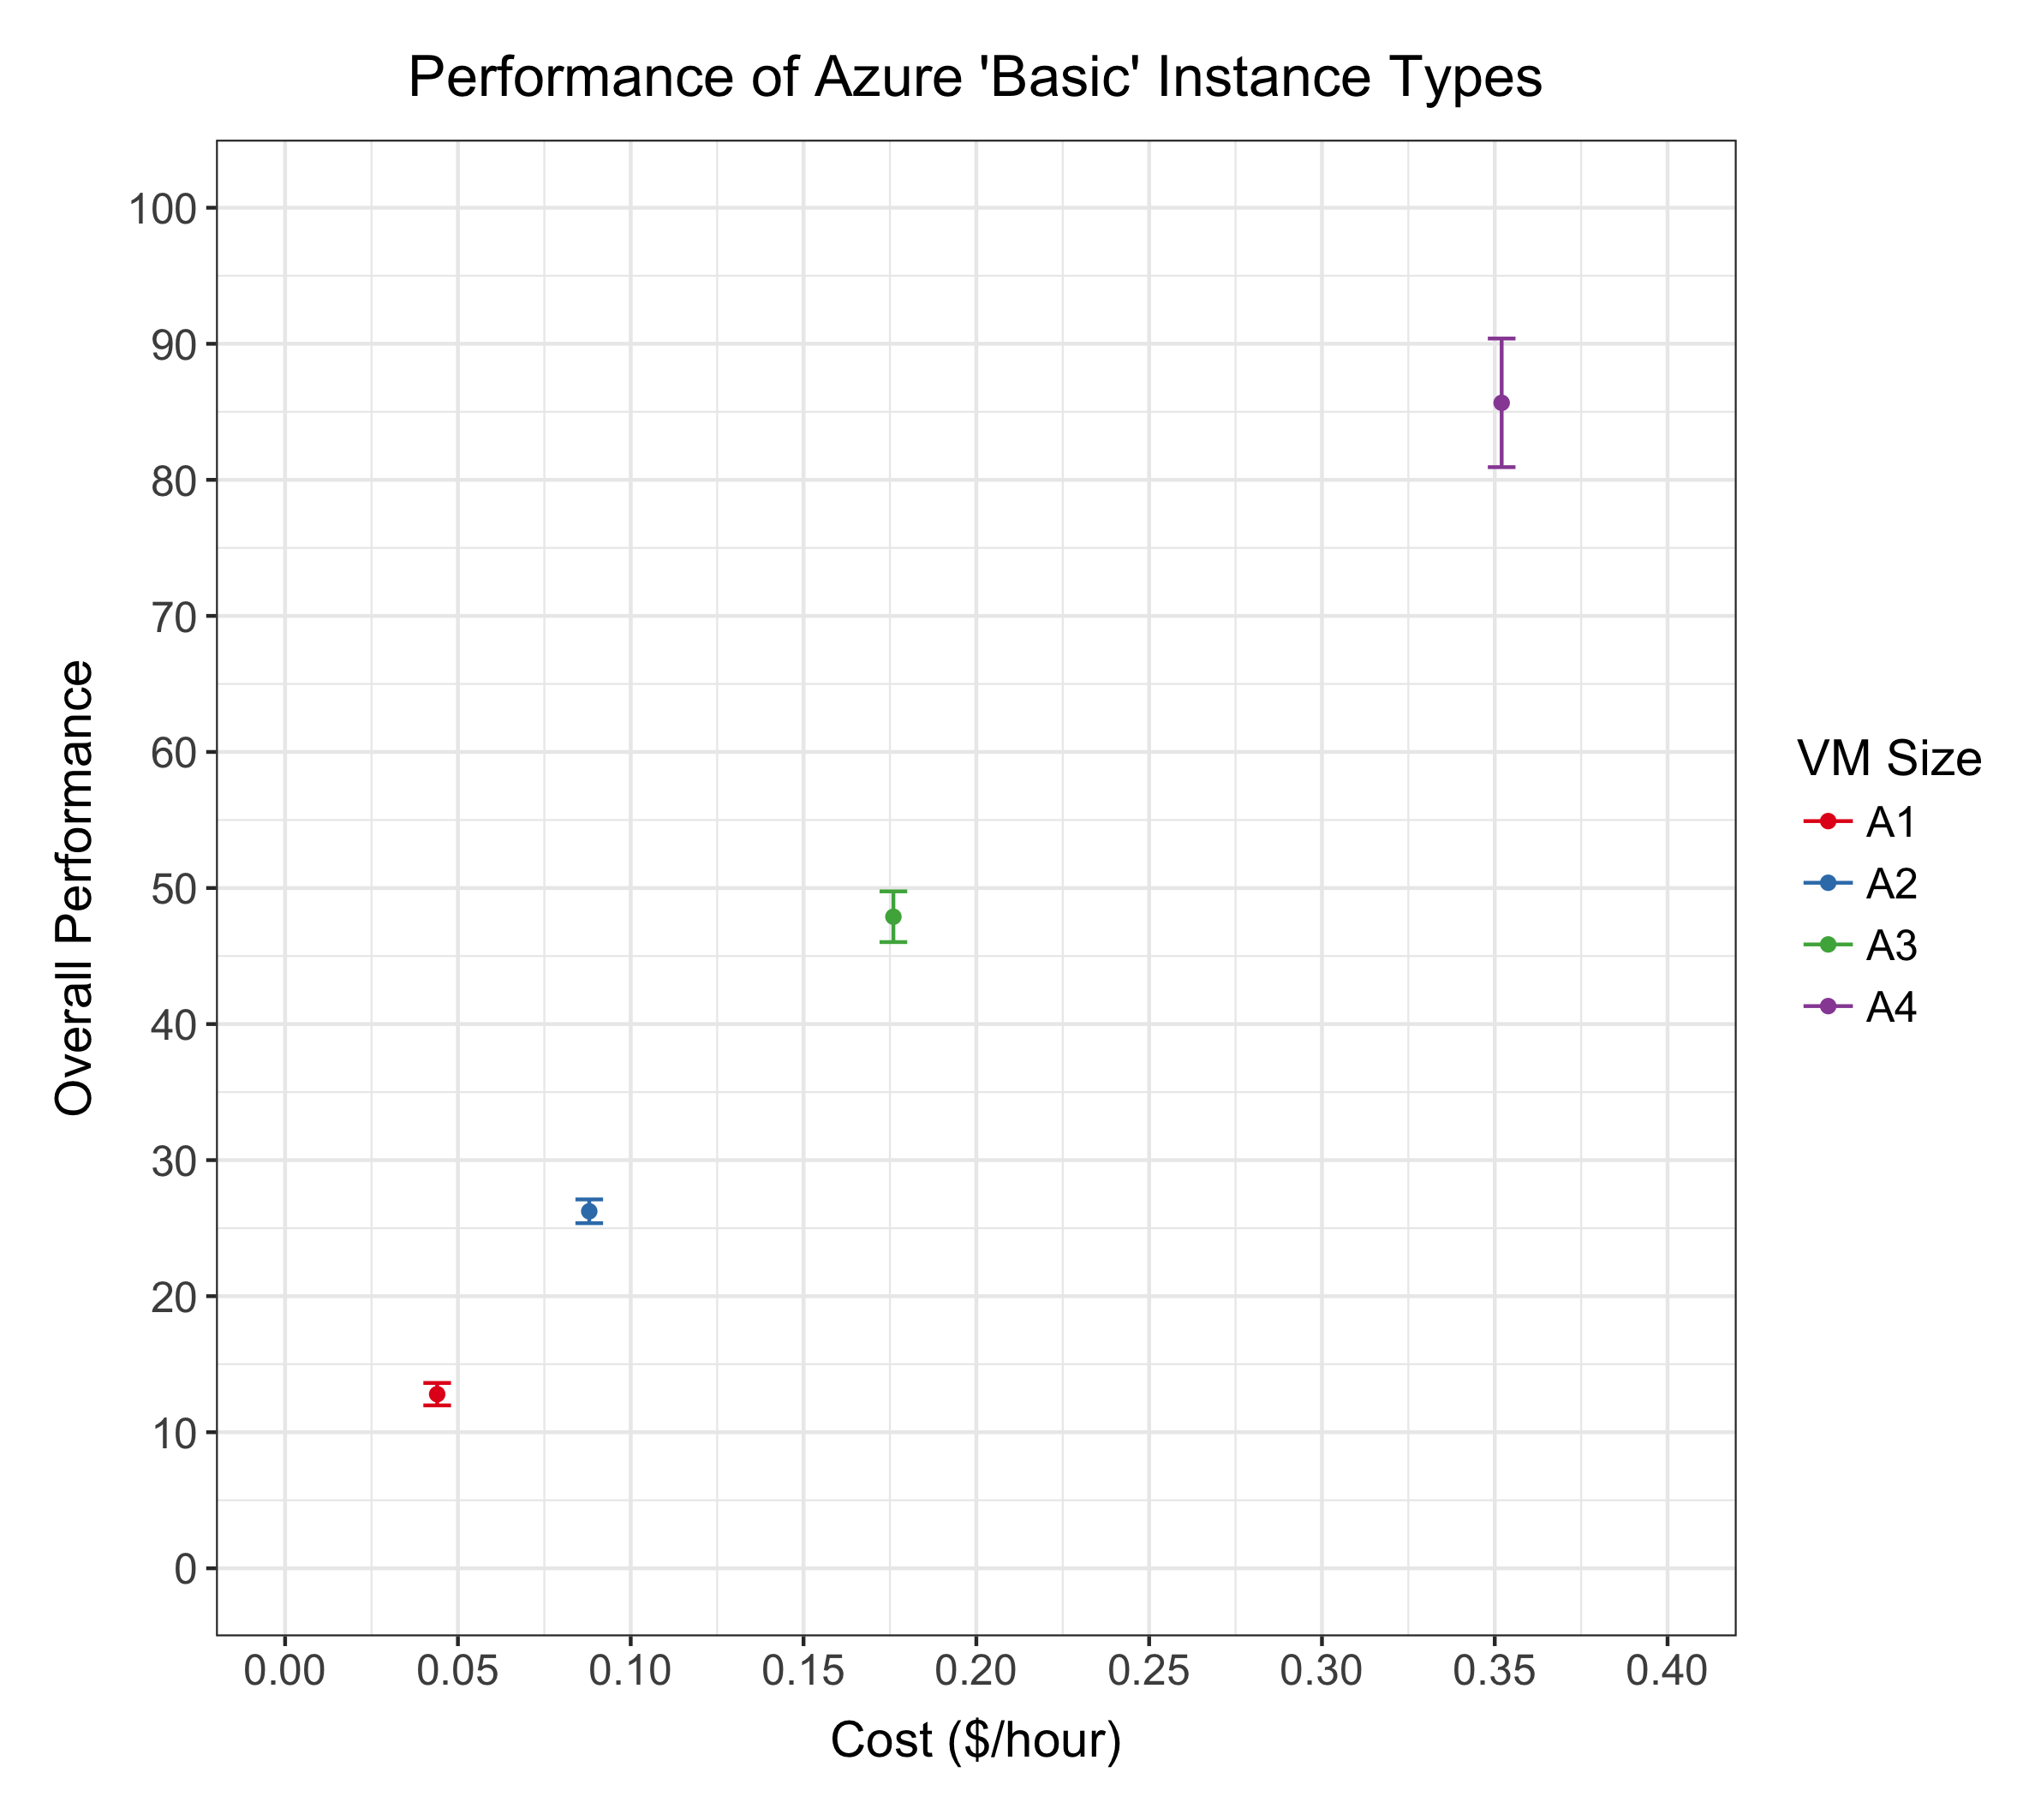
\includegraphics[width=\linewidth]{\graphs/data_azure_basic.png}
  \caption{Azure average basic instance performance results with variance}
  \label{fig:azure:basic}
\end{figure}
% =====================

The D-series VMs are Azure's optimised compute variants \cite{azurevmtype}. These have faster processors over the A-series variants, which should result in higher performance while keeping the number of cores the same. The results (table \ref{tab:azured}) show that this is the case, with every one of the D-series scoring nearly three times the amount of the equivalent basic tier model. The performance increase is in fact so great that the 4-core Standard\_D3 outperforms that of the 8-core Basic\_A4 by 32\% whilst also costing \$0.044/hour less for each VM. The same can be said for the 2-core Standard\_D2 when compared against the Basic\_A3 with a performance increase of 33\% and cost reduction of cost by \$0.022/hour per VM.

Performance results were also collected for the high memory variants of the D-series, Standard\_D11-13 where the JRE was created with more memory for testing. Whilst extra memory did not appear to have any effect on the performance results produced, the Standard\_D13 series showed a large amount of variability between different iterations when compared to its counterpart, the D4 (figure \ref{fig:azure:standard}). This may be somewhat a result of the time at which each iteration took place, as there was some difficulty in successfully provisioning D13 instances. The lack of performance benefit is likely due to the JRE being provided with significantly more memory than required, without the additional memory from these types of VMs -~\emph{``For all the JREs we have tested, 400 MB is sufficient for a system with 2 hardware threads''}~\cite{specjvmguide}.

% % Azure compute optimised variant Performance Table
% % =====================
\begin{table*}[!h]
  \caption{Performance result averages for Azure D-series across 5 iterations per instance type}
  \label{tab:azured}
  \begin{adjustbox}{width=\linewidth,center}
    \small
    % \csvautotabularcustom[respect all]{\data/data_average_azure_standard.csv}
    \begin{tabular}{|L{\lcollengthreg}|R{\rcolfive}|R{\rcolfive}|R{\rcolfive}|R{\rcolfive}|R{\rcolfive}|R{\rcolfive}|R{\rcolfive}|R{\rcolfive}|R{\rcolfive}|R{\rcolfive}|R{\rcolfive}|R{\rcolfive}|}
      \hline
VM Size & compiler & compress & crypto & derby & mpegaudio & scimark large & scimark small & serial & startup & sunflow & xml & Overall \\ \hline
d1 & 57.87 & 34.34 & 38.50 & 61.06 & 25.26 & 15.93 & 48.00 & 29.45 & 14.11 & 14.61 & 95.51 & 33.08 \\
d2 & 155.67 & 68.32 & 77.09 & 116.67 & 50.42 & 27.99 & 97.38 & 58.66 & 18.05 & 28.09 & 186.13 & 63.89 \\
d3 & 306.36 & 135.30 & 150.47 & 170.25 & 97.57 & 45.50 & 199.49 & 109.30 & 19.53 & 57.11 & 353.39 & 112.94 \\
d4 & 549.86 & 271.01 & 290.43 & 414.07 & 188.92 & 71.54 & 397.99 & 209.18 & 19.12 & 112.64 & 679.45 & 206.53 \\
d11 & 155.80 & 66.46 & 76.45 & 112.30 & 48.60 & 28.23 & 98.53 & 56.71 & 17.05 & 28.02 & 180.59 & 62.64 \\
d12 & 311.39 & 136.41 & 152.10 & 206.59 & 97.93 & 46.41 & 198.56 & 112.14 & 19.55 & 56.97 & 356.60 & 116.38 \\
d13 & 546.31 & 257.19 & 300.84 & 348.70 & 195.95 & 68.33 & 381.48 & 207.22 & 19.81 & 115.25 & 703.06 & 202.97 \\ \hline
    \end{tabular}

  \end{adjustbox}
\end{table*}
% % =====================

% Azure standard with variance
% =====================
\begin{figure}[ht]
  \centering
  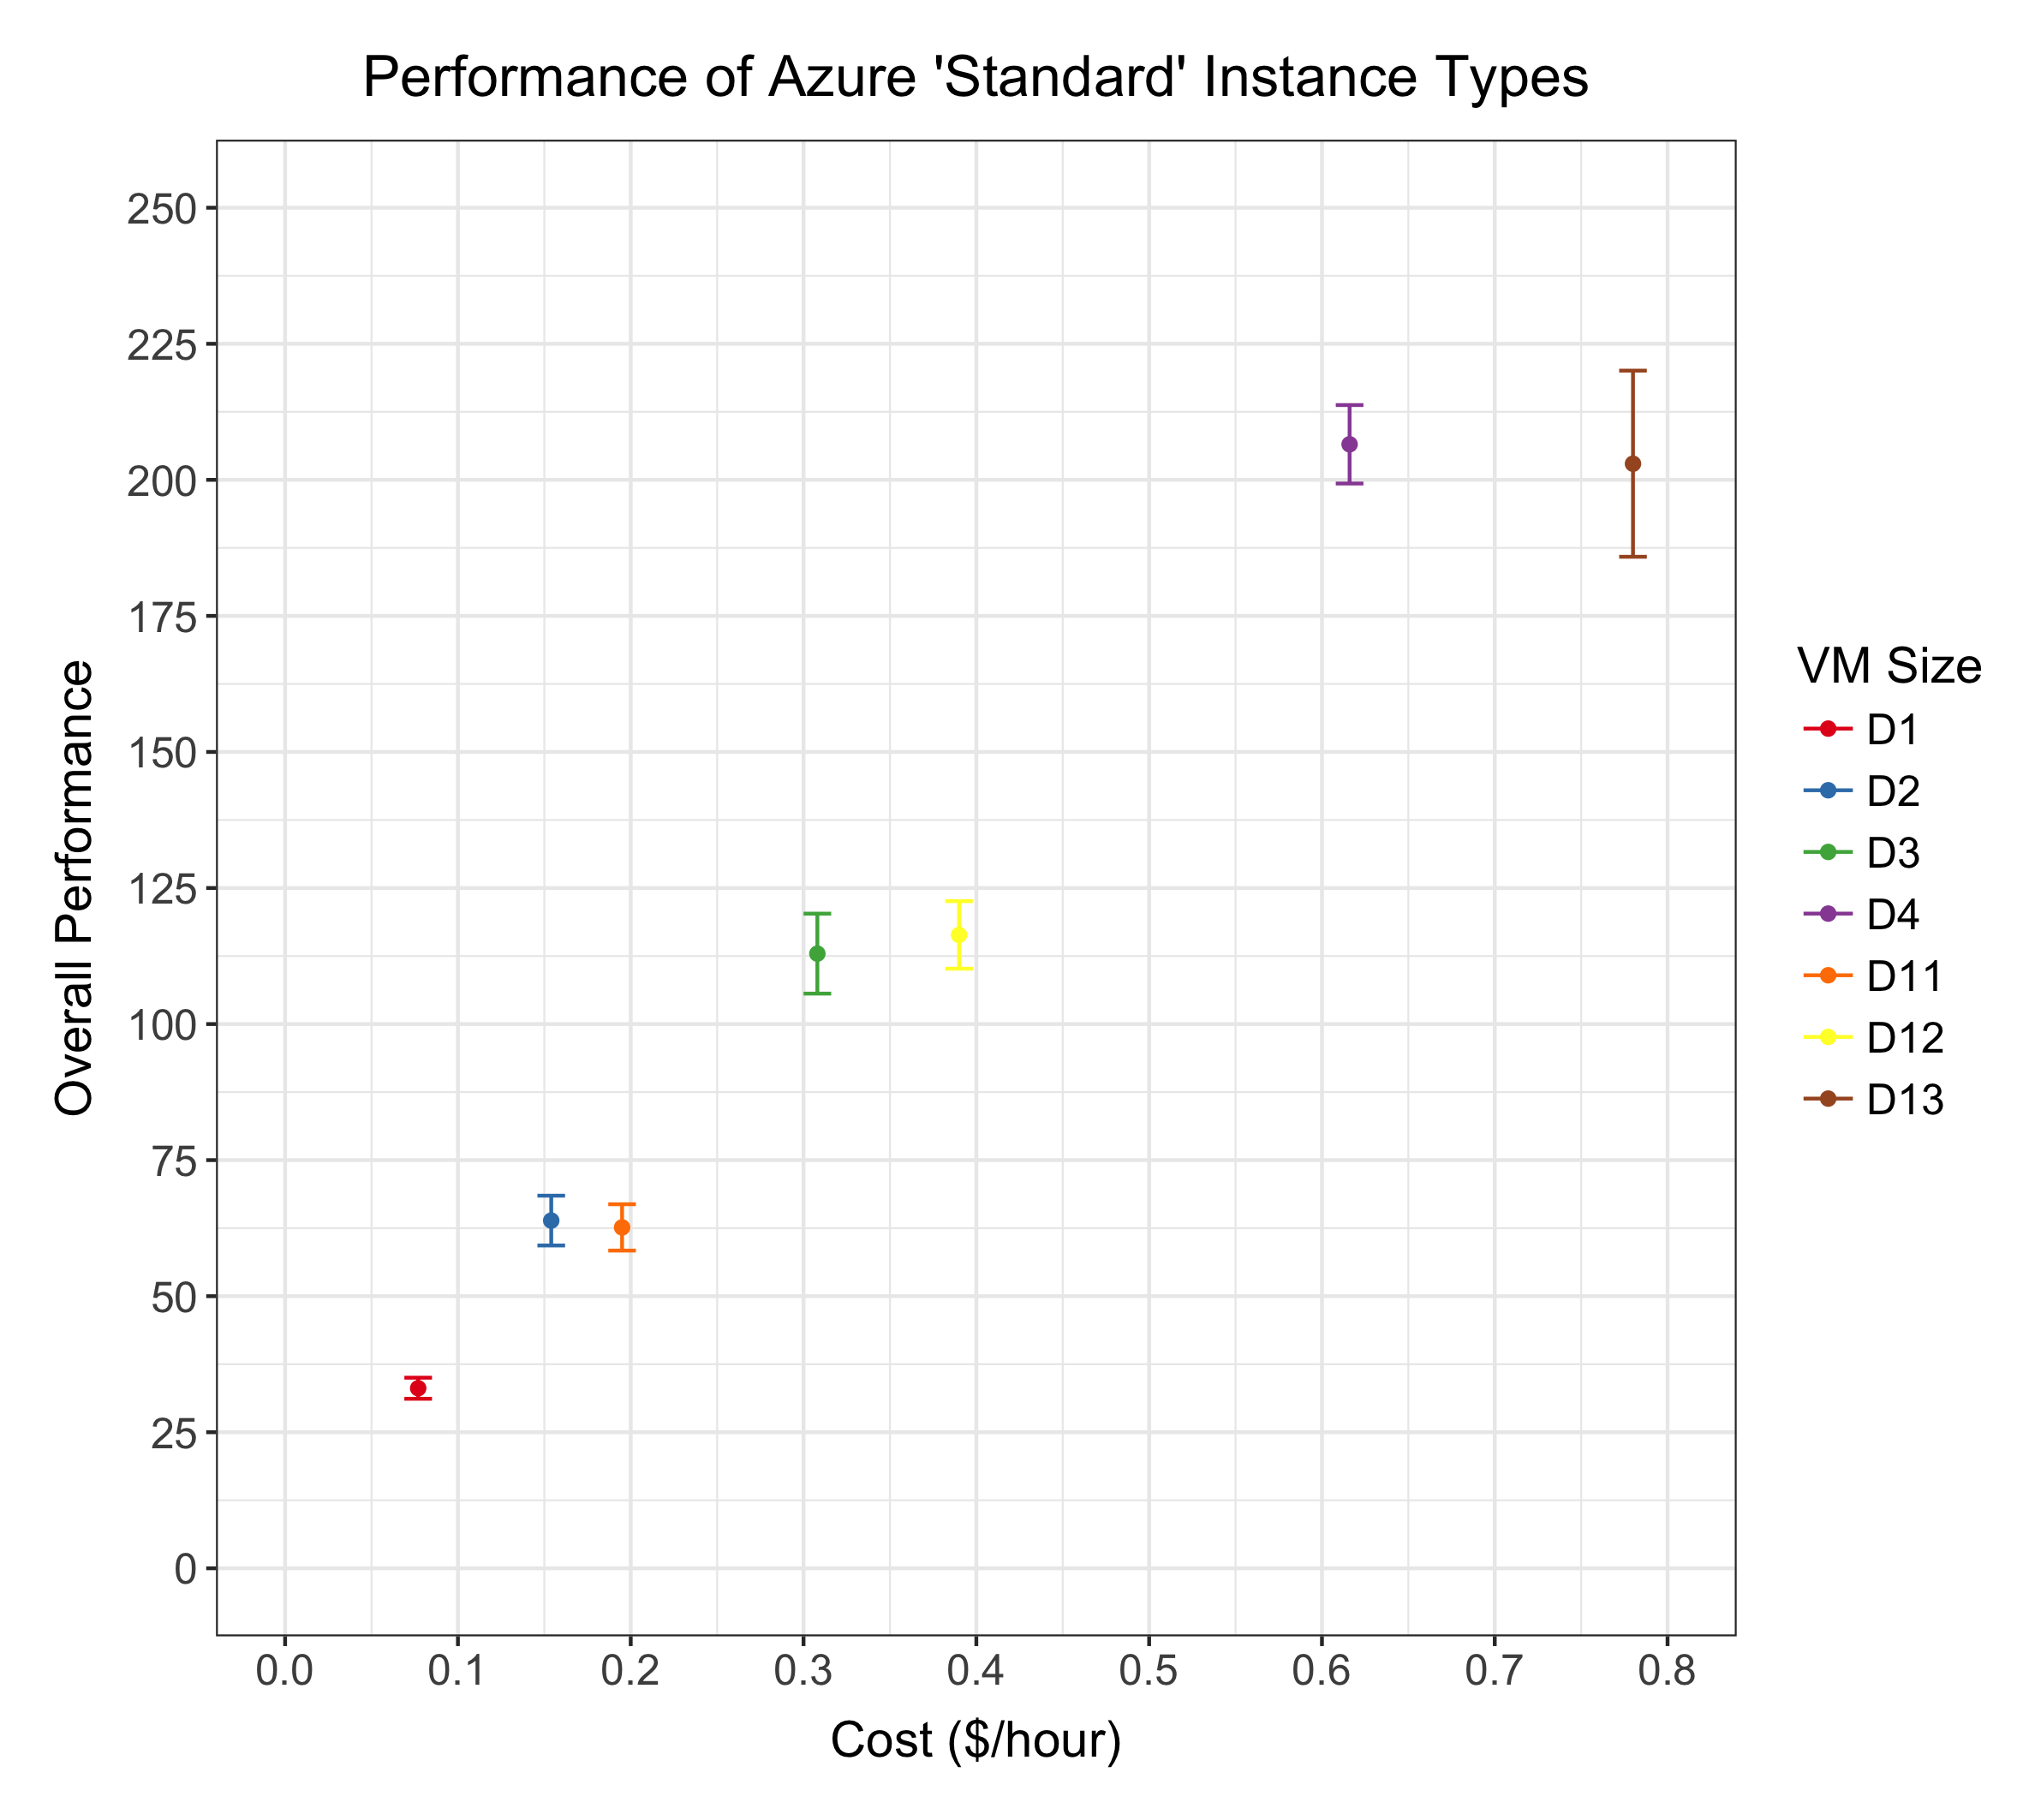
\includegraphics[width=\linewidth]{\graphs/data_azure_standard.png}
  \caption{Azure average standard instance performance results with variance}
  \label{fig:azure:standard}
\end{figure}
% =====================

Azure also offers a newer variant of the D-series with more powerful CPUs, named the Dv2-series, which are claimed to be 35\% faster than the original D-series \cite{azurevmtype}. The benchmark results (table \ref{tab:azuredv2}) show greatly increased performance on the Basic general purpose models, and an approximately 43\% increase in performance over the D-series across the different tiers for the SPECjvm2008 benchmark. A single core Standard\_D1\_v2 model outperforms the equivalent single core Basic\_A1 by nearly 4 times, whilst costing less than double the amount per hour. In fact, this single core Dv2 model has very similar performance to the results from the Basic\_A3 4-core machine, while costing less than half the amount per hour. This continues for the other Dv2 tiers, with the 2-core variant scoring only slightly less than the Basic\_A4 8-core VM whilst also costing substantially less.

When comparing the performance of the D-series with the Dv2-series, the cost is very important. Although the specifications of both of these series are identical for each tier, but with upgraded CPUs in the v2 series, the cost/hour of all Dv2-series are less than the equivalent D-series. This makes the increase in performance from the Dv2-series even more beneficial to a user, as there are no additional costs to taking advantage of this speed.

% % Azure compute optimised variant Performance Table
% % =====================
\begin{table*}[!h]
  \caption{Performance result averages for Azure Dv2-series across 5 iterations per instance type}
  \label{tab:azuredv2}
  \begin{adjustbox}{width=\linewidth,center}
    \small
    % \csvautotabularcustom[respect all]{\data/data_average_azure_standard_v2.csv}
    \begin{tabular}{|L{\lcollengthlarge}|R{\rcolfive}|R{\rcolfive}|R{\rcolfive}|R{\rcolfive}|R{\rcolfive}|R{\rcolfive}|R{\rcolfive}|R{\rcolfive}|R{\rcolfive}|R{\rcolfive}|R{\rcolsix}|R{\rcolfive}|}
      \hline
VM Size & compiler & compress & crypto & derby & mpegaudio & scimark large & scimark small & serial & startup & sunflow & xml & Overall \\ \hline
d1 v2 & 82.59 & 49.06 & 55.91 & 85.43 & 36.51 & 19.84 & 69.47 & 45.94 & 19.84 & 21.83 & 151.07 & 47.59 \\
d2 v2 & 230.55 & 98.84 & 113.81 & 160.84 & 72.52 & 32.95 & 139.14 & 90.96 & 25.26 & 41.50 & 284.28 & 91.45 \\
d3 v2 & 446.80 & 183.52 & 216.06 & 242.91 & 135.68 & 47.22 & 268.74 & 164.49 & 27.90 & 77.89 & 535.10 & 156.33 \\
d4 v2 & 846.63 & 370.90 & 422.39 & 615.61 & 267.04 & 64.25 & 522.43 & 317.23 & 27.72 & 157.77 & 1048.73 & 286.37 \\
d11 v2 & 233.13 & 96.07 & 112.59 & 167.98 & 70.65 & 35.96 & 138.40 & 86.64 & 25.30 & 39.61 & 278.92 & 91.14 \\
d12 v2 & 444.79 & 183.70 & 215.07 & 281.57 & 136.92 & 50.54 & 267.60 & 164.73 & 27.94 & 78.24 & 532.88 & 159.94 \\
d13 v2 & 575.80 & 367.98 & 412.32 & 588.54 & 266.92 & 62.29 & 509.81 & 311.86 & 27.92 & 156.94 & 1054.62 & 272.91 \\ \hline
    \end{tabular}
  \end{adjustbox}
\end{table*}
% % =====================

% % Azure standard_v2 with variance
% % =====================
% \begin{figure}[ht]
%   \centering
%   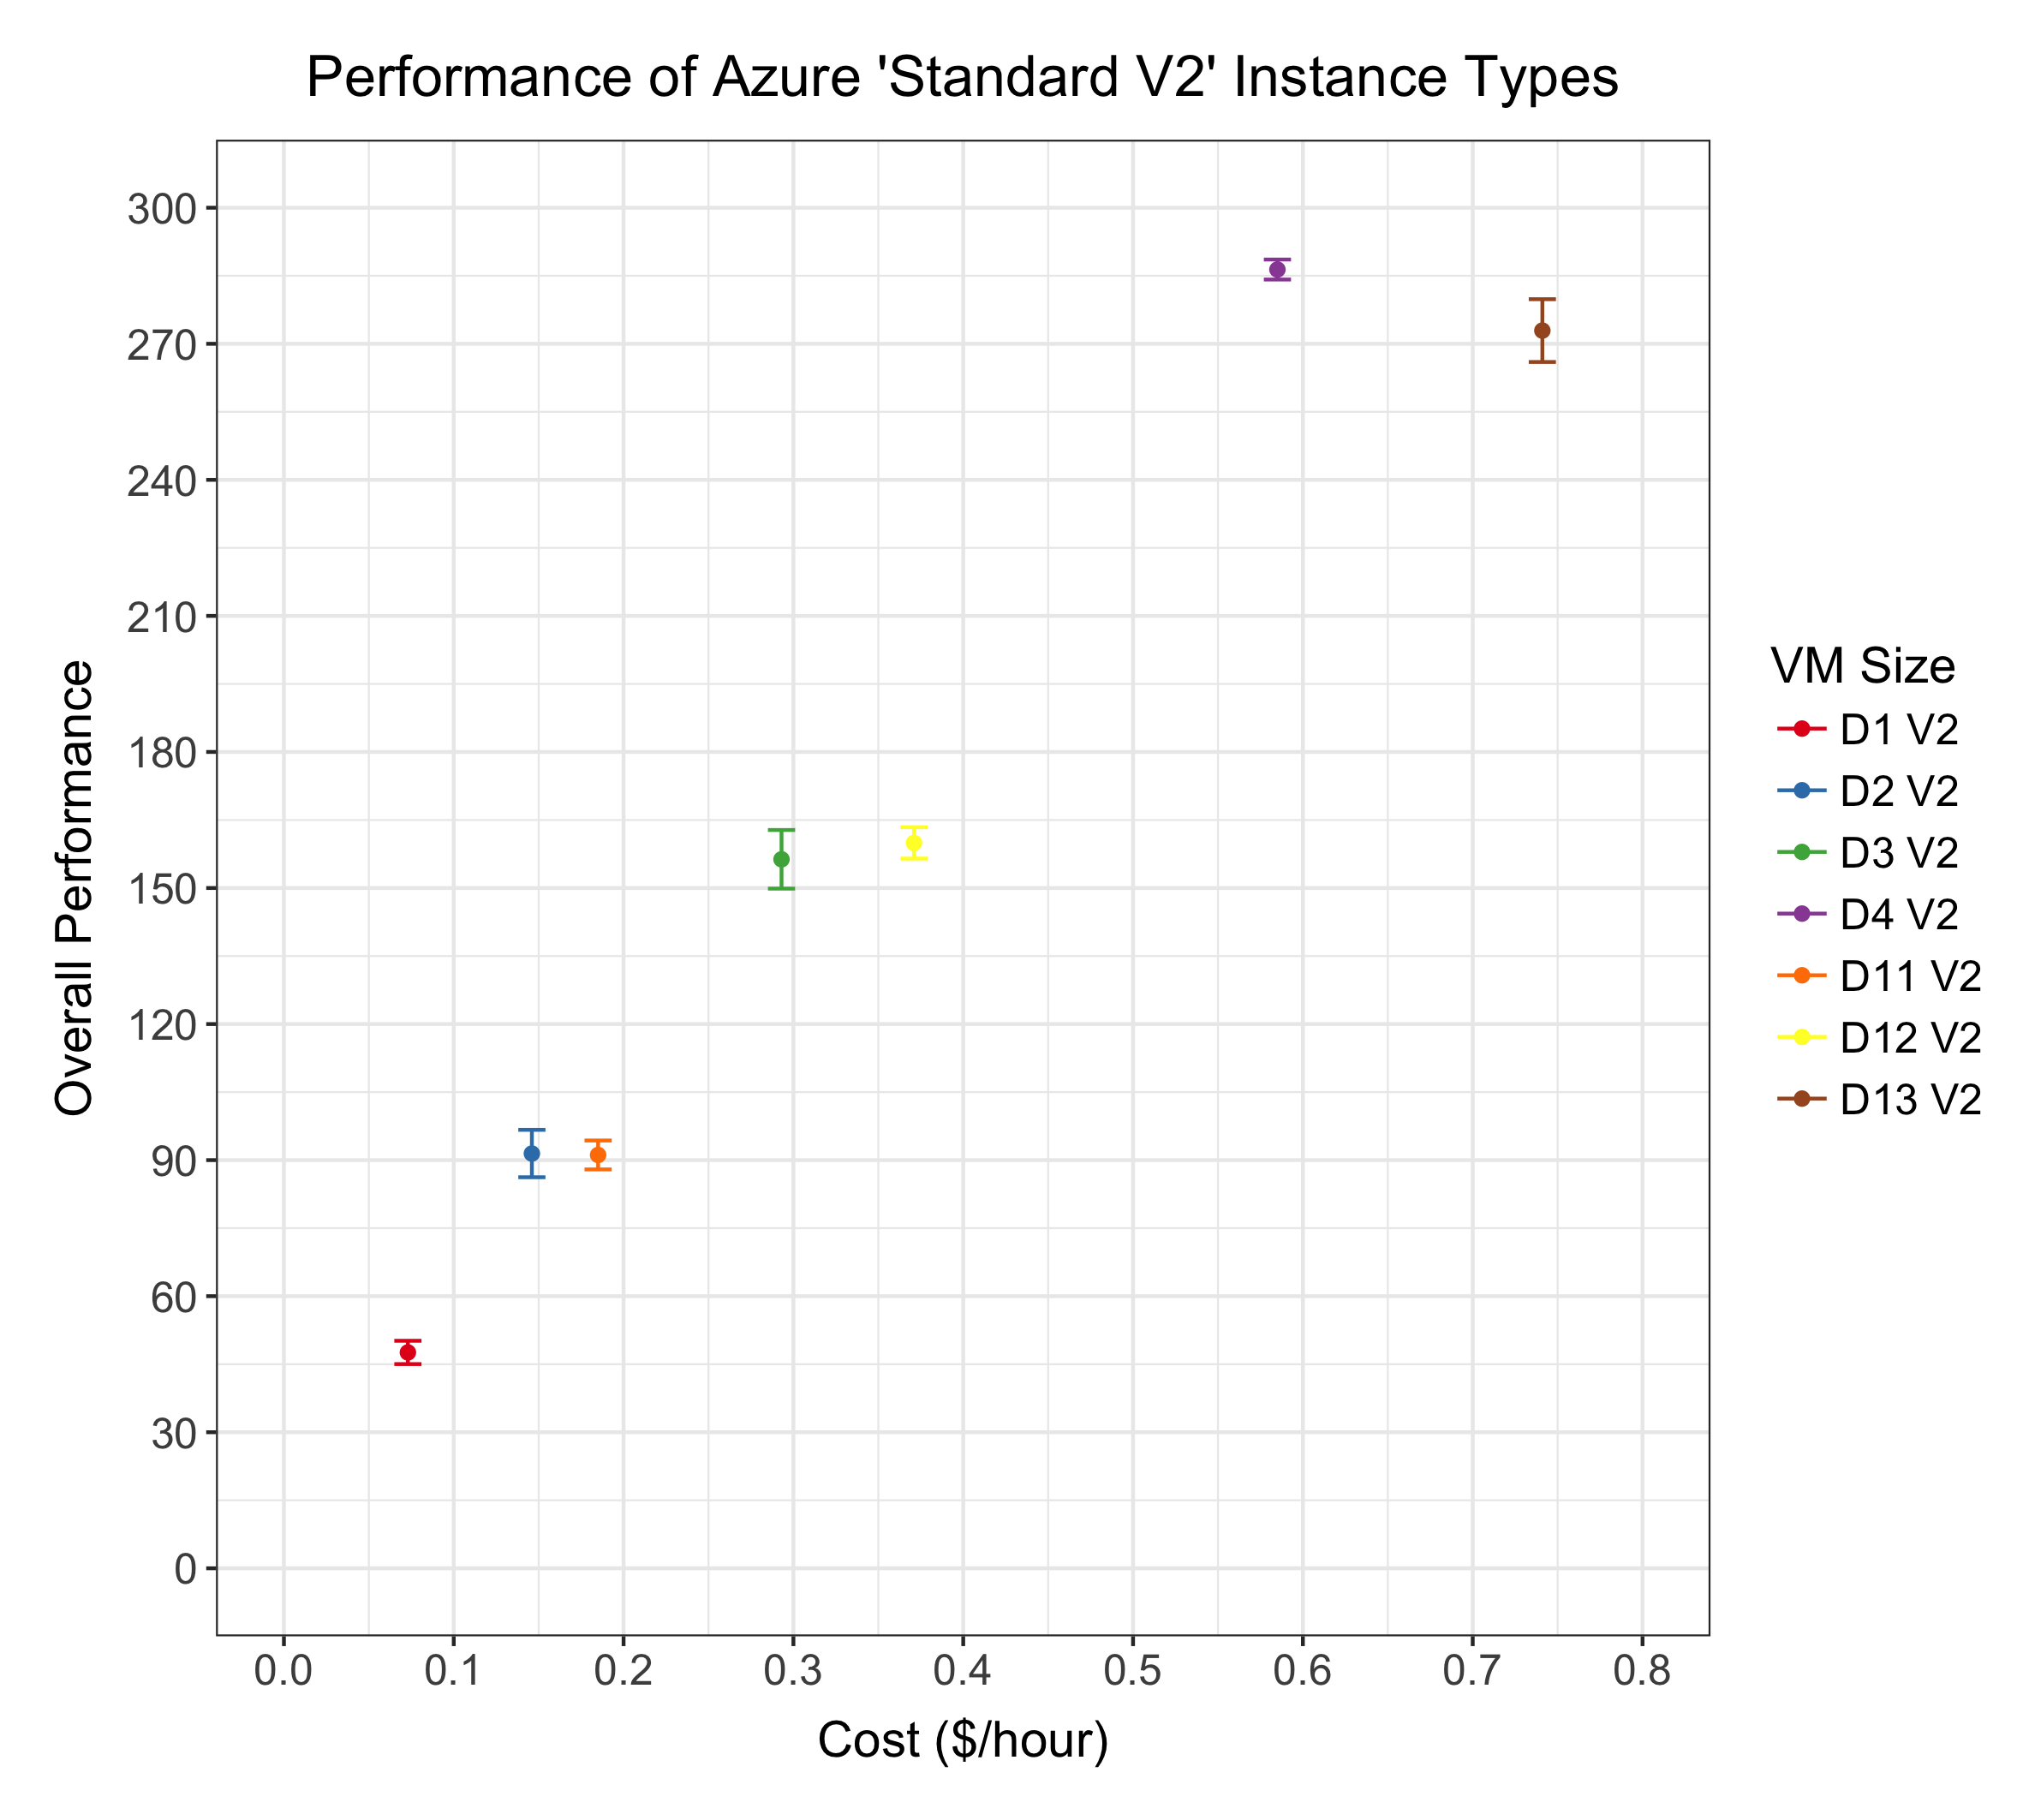
\includegraphics[width=\linewidth]{\graphs/data_azure_standard_v2.png}
%   \caption{Azure average standard v2 instance performance results with variance}
%   \label{fig:azure:standard:v2}
% \end{figure}
% % =====================

% % Graph comparison of Azure types
% % =====================
% \begin{figure}[ht]
%   \centering
%   \includegraphics[width=\linewidth]{azurechart.png}
%   \caption{Comparison of Azure tier performance}
%   \label{fig:azurechart}
% \end{figure}
% % =====================



\subsubsection{Amazon Elastic Compute Cloud Results}\label{sec:eval:awsresults}

The second set of data (table \ref{tab:ec2}) is collected from Amazon's EC2, running the benchmark on several T2 general purpose instances, newer generation general purpose M4 instances, alongside some compute optimised C4 instances \cite{awsvmtype}. When looking at the results from T2 instances, an increase in performance can be seen from one tier to the next one, which is generally expected when the hardware specification of the VMs increases also. However, from a t2.micro to a t2.small, the number of cores remains the same while the memory increases. Although this is the case, the JRE was provided with the same amount of memory for both of these benchmark runs, and so the capacity increase should not have affected the results for the runs.

The same approximately 50\% increase in performance occurs between the\linebreak t2.medium and t2.large VMs where there is only 2-cores available (figure \ref{fig:aws:t2}). This increase in performance is most likely due to the nature of T2 instances as burstable performance instances \cite{awsvmtype}. Although the number of cores remains the same between these tiers, the number of credits increases so that the CPU can burst above the baseline more frequently. This ability to burst will have a direct effect on the benchmark results. The largest increase in performance however is when switching between the single core system of a t2.small and the 2-core t2.medium instance type, where the latter scores very nearly double of the former, whilst the cost/hour increases by exactly double.

% % AWS Performance Table
% % =====================
\begin{table*}[!h]
    \caption{Performance result averages for Amazon EC2 across 5 iterations per instance type}
    \label{tab:ec2}
  \begin{adjustbox}{width=\linewidth,center}
    \small
    % \csvautotabularcustom[respect all]{\data/data_average_aws.csv}
    \begin{tabular}{|L{\lcollengthlarge}|R{\rcolfive}|R{\rcolfive}|R{\rcolfive}|R{\rcolfive}|R{\rcolfive}|R{\rcolfive}|R{\rcolfive}|R{\rcolfive}|R{\rcolfive}|R{\rcolfive}|R{\rcolfive}|R{\rcolfive}|}
      \hline
VM Type & compiler & compress & crypto & derby & mpegaudio & scimark large & scimark small & serial & startup & sunflow & xml & Overall \\ \hline
c4 large & 156.55 & 68.66 & 70.71 & 136.17 & 49.26 & 28.46 & 106.12 & 55.38 & 25.41 & 28.05 & 179.60 & 66.31 \\
c4 xlarge & 311.31 & 136.74 & 143.20 & 261.17 & 99.63 & 54.34 & 211.10 & 109.67 & 30.65 & 55.99 & 357.84 & 125.58 \\
c4 2xlarge & 556.12 & 276.84 & 287.60 & 504.95 & 198.13 & 82.04 & 410.20 & 211.22 & 32.95 & 112.61 & 717.18 & 227.19 \\
m4 large & 138.10 & 59.97 & 59.49 & 117.59 & 41.31 & 26.21 & 89.82 & 47.44 & 21.91 & 23.80 & 153.39 & 57.18 \\
m4 xlarge & 270.11 & 118.08 & 119.11 & 224.29 & 83.69 & 48.03 & 182.14 & 92.81 & 26.18 & 47.56 & 303.43 & 107.35 \\
m4 2xlarge & 521.63 & 238.94 & 237.17 & 437.86 & 167.46 & 75.07 & 354.09 & 180.74 & 27.93 & 94.90 & 608.58 & 196.38 \\
t2 micro & 81.40 & 47.04 & 39.14 & 15.49 & 3.59 & 2.18 & 6.92 & 5.27 & 19.78 & 2.11 & 13.47 & 11.08 \\
t2 small & 74.45 & 47.49 & 48.64 & 37.44 & 6.99 & 4.23 & 13.84 & 8.49 & 19.20 & 4.12 & 25.04 & 17.38 \\
t2 med & 209.83 & 93.90 & 104.25 & 87.84 & 13.34 & 8.19 & 27.74 & 15.64 & 25.48 & 8.25 & 49.00 & 34.67 \\
t2 large & 228.43 & 93.14 & 110.68 & 179.16 & 39.32 & 12.29 & 41.03 & 27.56 & 26.30 & 12.10 & 85.51 & 51.13 \\ \hline
    \end{tabular}
  \end{adjustbox}
\end{table*}
% % =======================

% EC2 t2 with variance
% =====================
\begin{figure}[ht]
  \centering
  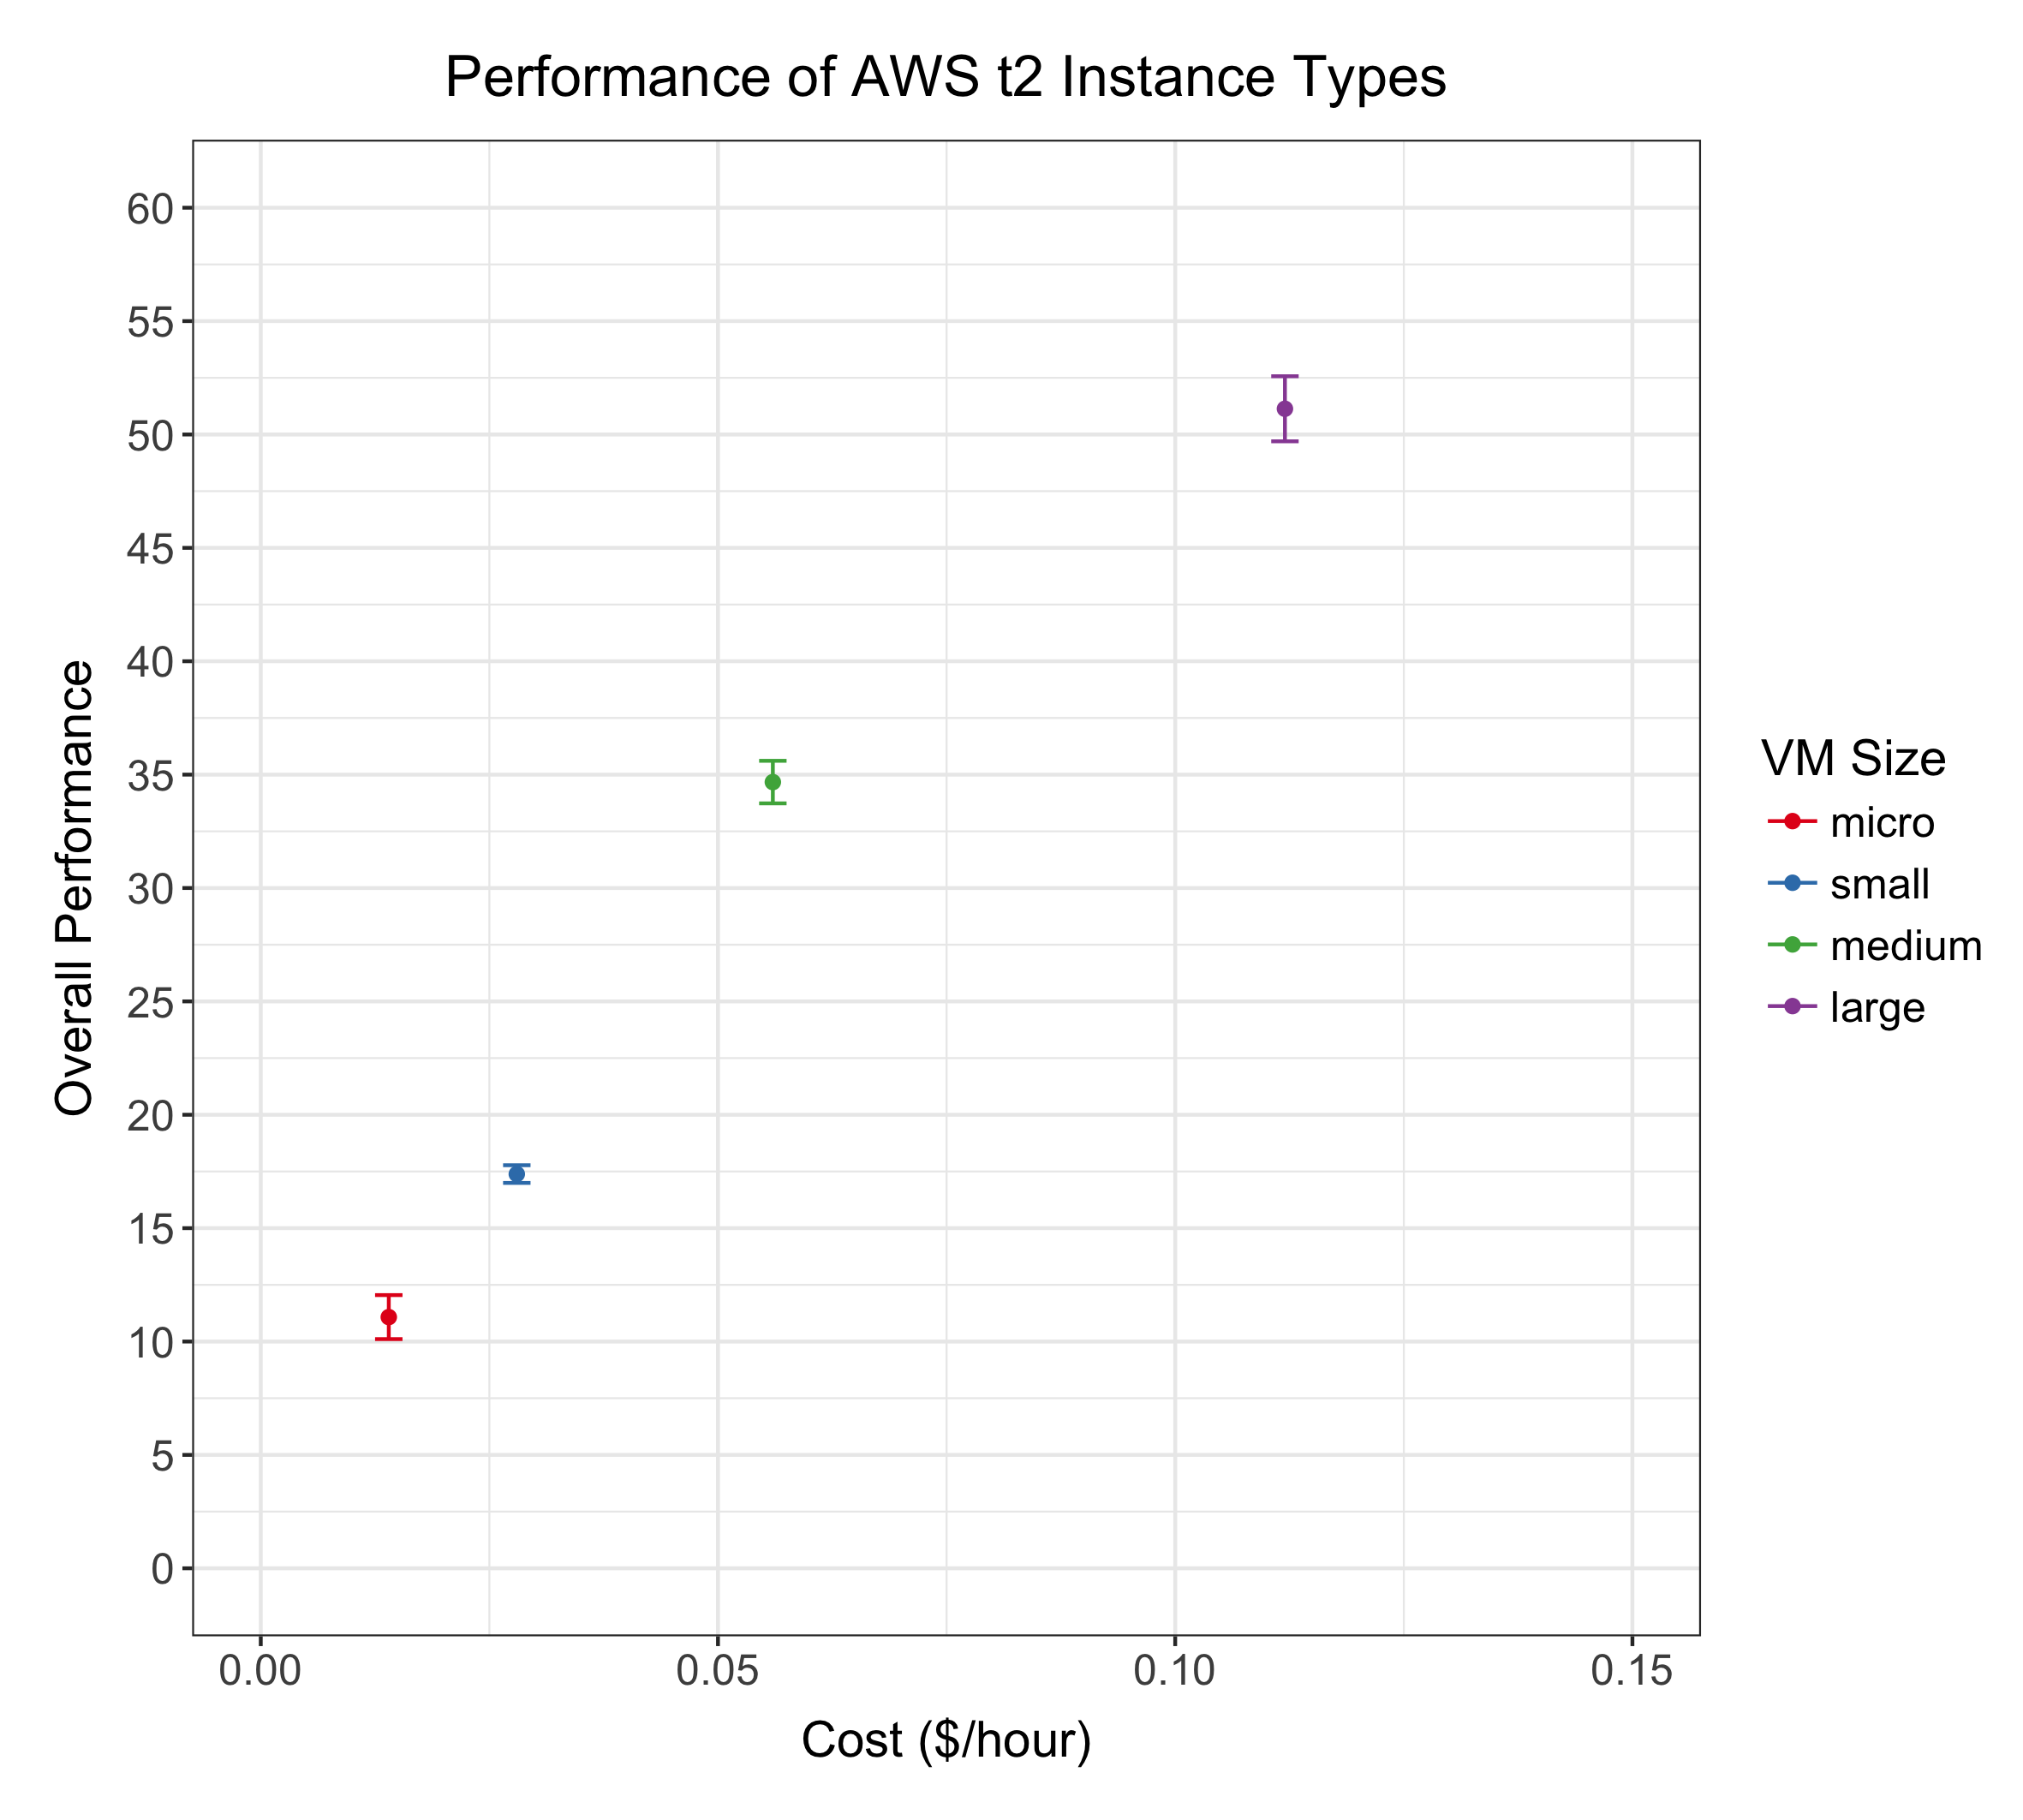
\includegraphics[width=\linewidth]{\graphs/data_aws_t2.png}
  \caption{EC2 t2 instance average performance results with variance}
  \label{fig:aws:t2}
\end{figure}
% =====================

The newer general purpose M4 instance types start with a baseline specification of 2-cores and 8GB memory capacity, alike other large instance types. This m4.large instance outperforms the equivalent t2.large instance by a mere 12\%, when the cost increase from \$0.112 to \$0.132 is an increase by 17\%. The reason for the difference in performance being so minor could be due to the T2s burstable performance. Each T2 VM receives CPU credits at the beginning of each hour, which allow them to burst above the baseline core usage \cite{awsvmtype}. The full benchmark run time is approximately 2.25 hours, and is likely to be using near 100\% utilization of that which is available at all times. For the first two hours of running, the benchmark will use up the available credits, and run at baseline for the remaining time before more credits are provided at the hourly boundary. For the last hour slot where only 25\% of the time is used, the benchmark may be able to burst with the available credits for the remaining duration of the benchmark. If when bursting, the performance of this t2.large instance was greater than that of an m4.large, but far lower when no credits were available and running at baseline, the expected performance would be within the region of that which is seen. The startup and compiler tests which run towards the beginning of the benchmark, while credits would be available to a T2 instance, have greater results for the T2 instance than the M4, whereas others such as scimark and serial, have superior performance on the M4 instance. If the benchmark ran over the entire VM hour slots provided with high utilization, the scores would likely be worse than at present due to running out of credits in the third hour and running at baseline for the remainder of the hour.

% % Graph comparison of EC2 types
% % =====================
% \begin{figure}[ht]
%   \centering
%   \includegraphics[width=\linewidth]{ec2chart.png}
%   \caption{Comparison of EC2 tier performance}
%   \label{fig:ec2chart}
% \end{figure}
% % =====================

% % EC2 variability
% % =====================
% \begin{figure}[ht]
%   \centering
%   \includegraphics[width=0.8\linewidth]{ec2_variability.png}
%   \caption{EC2 average performance results with variance}
%   \label{fig:ec2variability}
% \end{figure}
% % =====================

Amazon also has a compute optimised instance selection within the C4 series which have the highest performing CPUs out of the different series. Across the board these perform around 16\% better at the benchmark than the M4 series for each instance type, whilst costing around 10\% less. This reduction in cost is most likely due to the compute optimised variants having less than half the memory capacity of the general purpose M4s. As the benchmark does not require large amounts of memory, the additional memory capacity of the M4 instances does not have much, if any impact on the results seen. It is likely that a high-memory consuming workload would perform better on M4 instances than the C4 series, as the improved CPU performance would weigh less when compared to the memory capacity gained. When comparing the C4 series to a T2 instance at similar capacity, in this case c4.large and t2.medium, there is a less than double performance improvement with slightly more than double the cost/hour. If these instances are compared by scores excluding the single threaded startup test, the performance per cost is nearly equivalent. Moving from one C4 instance to the next, the performance results do not quite keep up with the cost and core count increase. However, when comparing a overall result without the influence of the single threaded `startup' test, the performance per cost increases approximately linearly.


\subsubsection{Comparison of Azure and EC2}

The results for similar specification VM instances across both of the cloud providers showed near same performance for some of the fixed instances (figure \ref{fig:bothchart}). An example of which is Standard\_D2 and m4.large, both 2-core instance types with 7GB and 8GB of memory respectively, that were within an average composite score of $60\pm3$, with the D2 taking the lead. Similar results are also seen between the Standard\_D3 and m4.xlarge, with Azure's D3 marginally outperforming again. Although this is the case, Azure's D-series does have a higher proportion increase in cost per hour than performance gained, when looking at the M4 equivalent of Amazon's EC2. The newer optimised compute Dv2-series also outperforms the EC2 equivalent, the C4 instance types, with 2-core D2\_v2 scoring a 38\% higher result than the equivalent c4.large, with only a 23\% increase to cost. Other D2v2 instances however have performance increases more proportionate to the cost/hour increase. One of the main benefits to Azure's higher tier offerings is that of a single core machine. Neither the M4, or C4 instance types provide a single core machine, whereas Azure has both the D-series Standard\_D1 and Dv2-series Standard\_D1\_v2. For any workloads that are only designed to run in a single thread, if it is preferred that these run on the newer compute optimised or general purpose EC2 instances, they should be batch loaded onto the system to make the most of available virtual cores.

% Graph comparison of EC2 and Azure types
% =====================
\begin{figure}[ht]
  \centering
  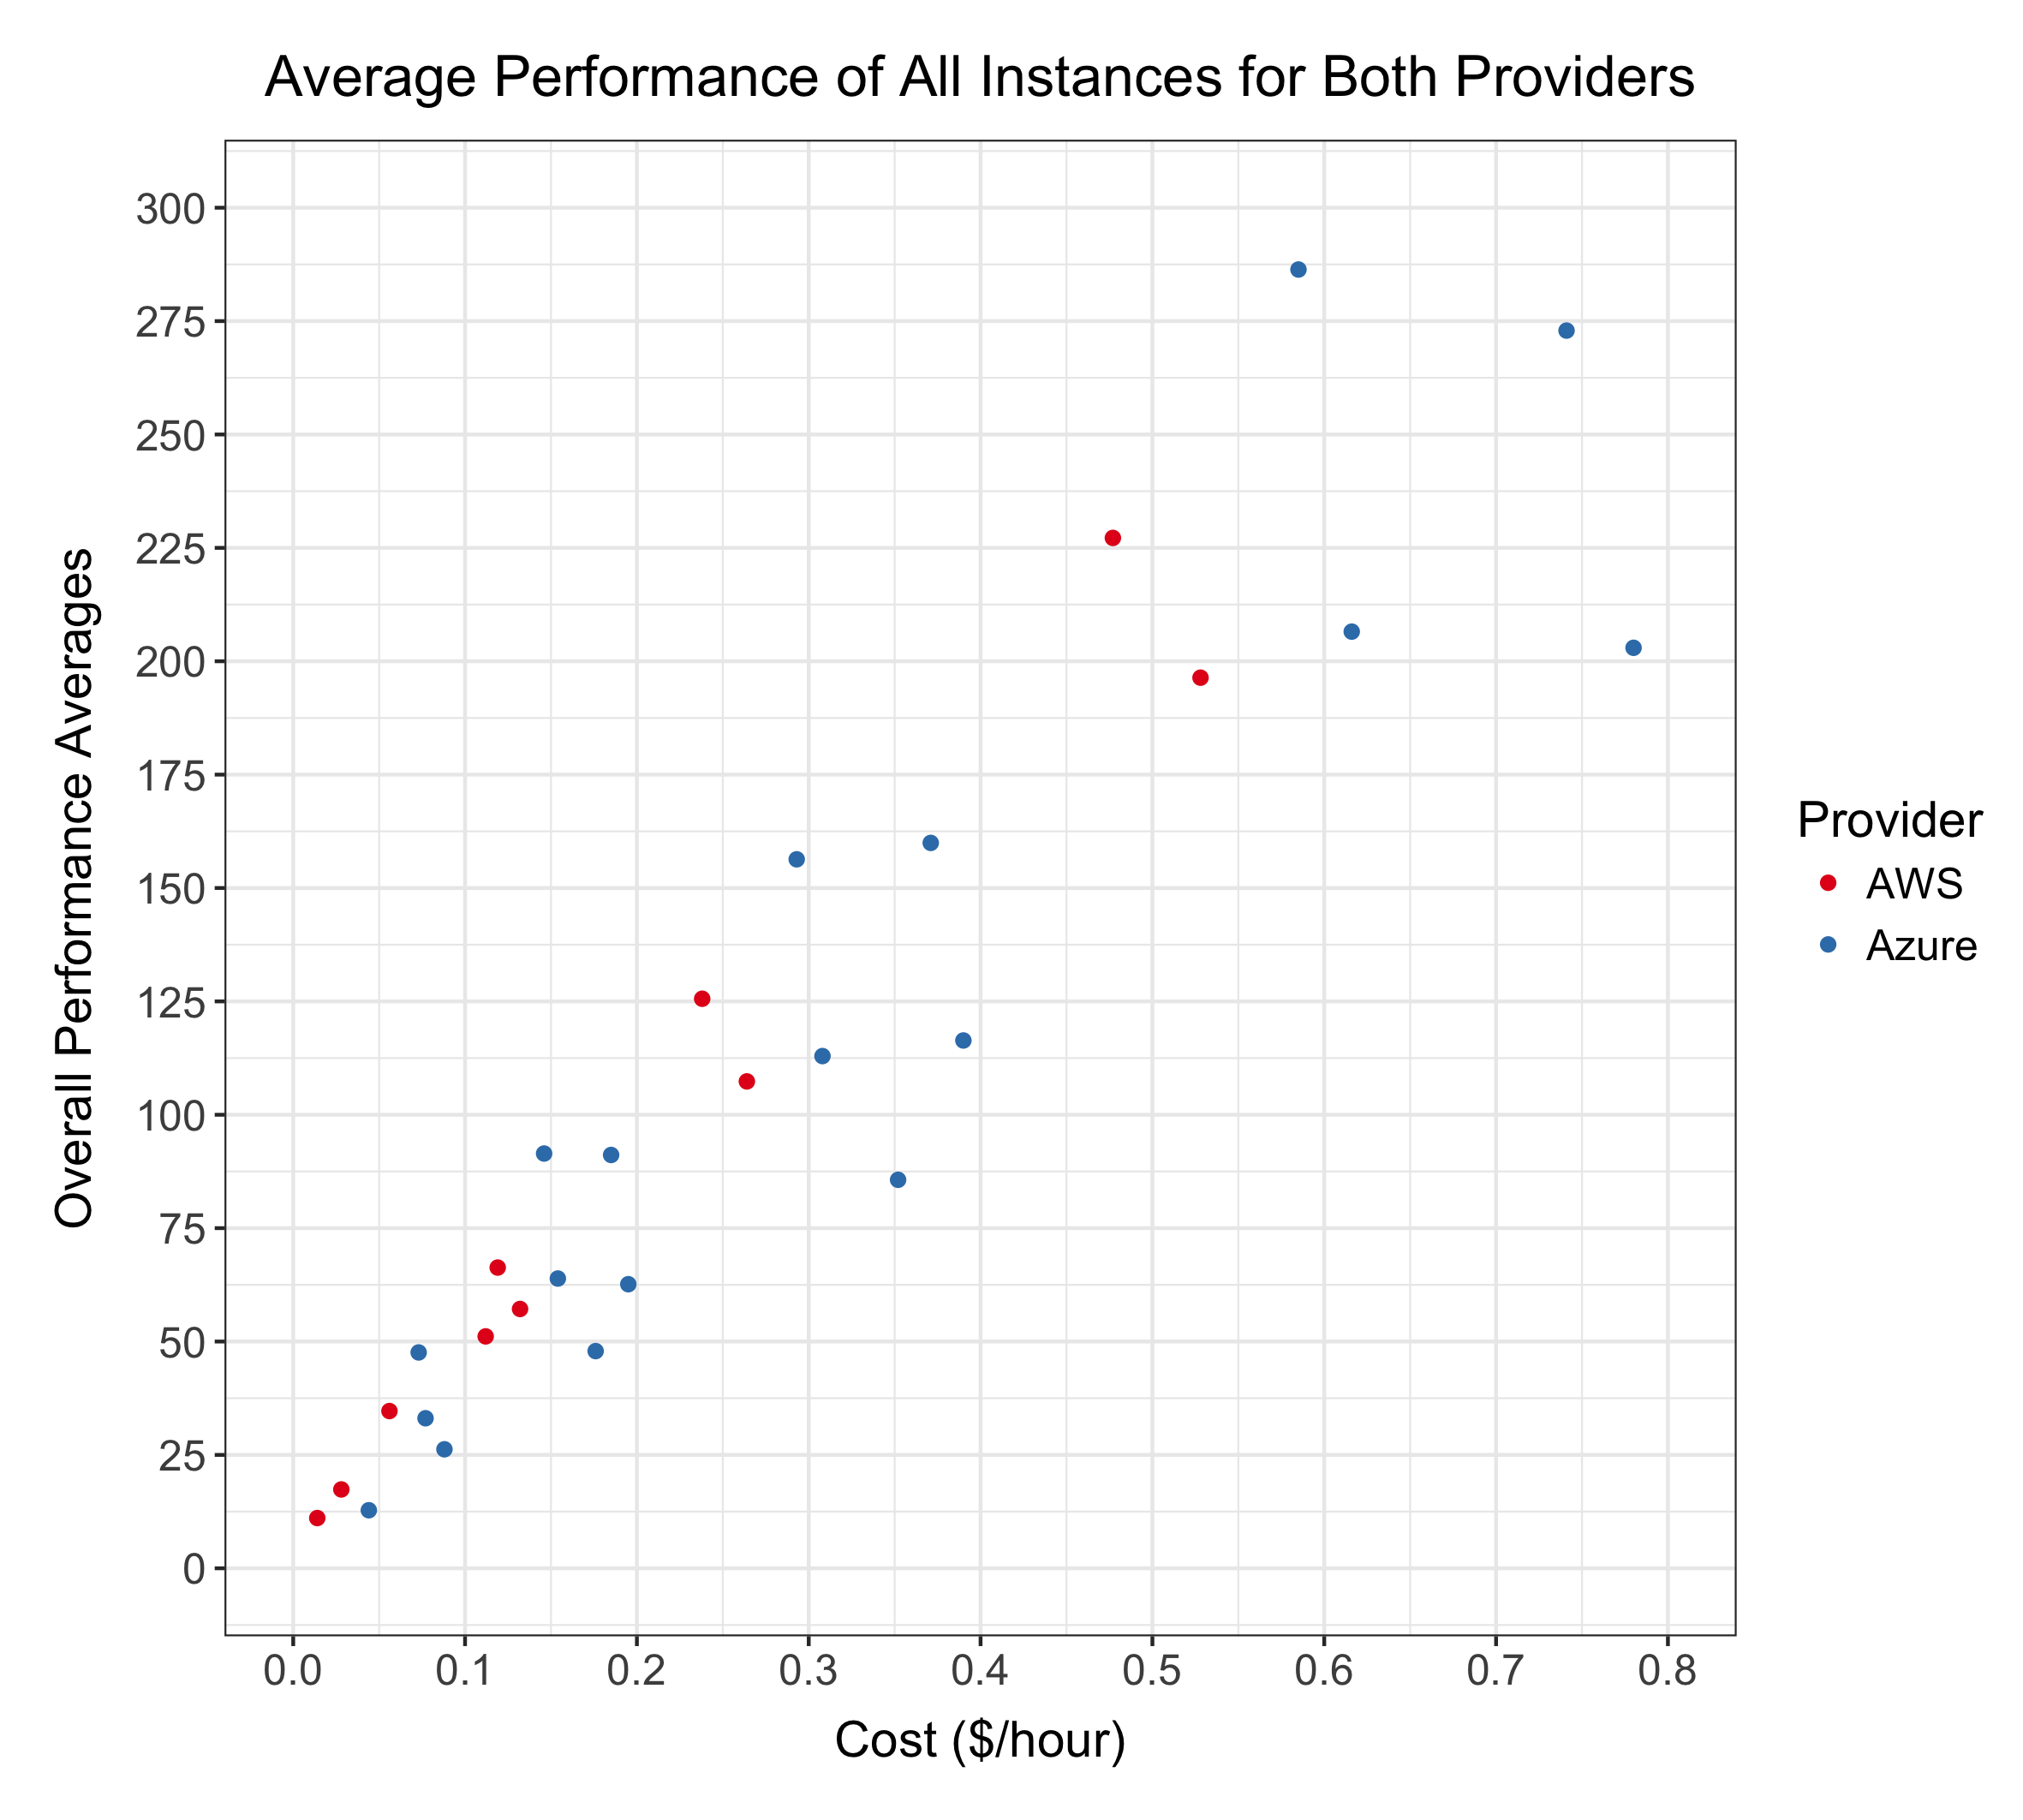
\includegraphics[width=\linewidth]{\graphs/data_both.png}
  \caption{Comparison of Azure and EC2 performance}
  \label{fig:bothchart}
\end{figure}
% =====================

Amazon's burstable T2 instance types perform well for the lower tier instances. Azure's A1 performs slightly worse to that of a t2.micro instance, where the cost of the micro is considerably less. The single core t2.small outperforms the Standard\_A1 whilst still costing \$0.016 cheaper per hour. The results obtained however may be skewed in favour of the burstable performance instances, due to the nature of the task being run and the length of the benchmark execution; as discussed in section \ref{sec:eval:awsresults}. When the T2 instances have CPU credits available, the bursting performance is high, with similar results to the optimised compute D2\_v2 Azure instance type and A4 8-core in the initial compiler test, at lower cost. For this reason, the T2 would perform the best for cost if performance requirements are variable and follow more of a `bursty' pattern. If the workload has high computation requirements over an extended period of time, the higher core compute optimised machines may be better, assuming the workload runs on multiple threads. If this workload requires large utilization but is single threaded, the newer higher clock speed instance types would result in superior performance.

\subsubsection{Extended Testing}\label{sec:eval:extended}

Some workloads may be single threaded, and therefore unable to benefit from the additional cores that a virtual machine offers. This limits the number of options for these sorts of tasks on current cloud offerings, as the price of multicore systems represents the performance gained from additional cores. However, it may be possible to batch load a number of single-threaded tasks on to a multicore instance type. If the performance of a single thread on a multiple core instance is higher than that of a single core system, and the price per core is the same, it may be worth loading a single threaded job per core on the multicore system to take advantage of the higher performance. SPECjvm2008 supports running in single threaded mode\cite{specjvmguide}, and so results have been collected of the performance across the multicore variants of both the D-series and Dv2-series. As the previously collected results were not greatly influenced by high memory instance types, the D11-13 VM types have been excluded from the testing process.

% % Azure single threaded Performance Table
% % =====================
\begin{table*}[!h]
  \caption{Single-threaded performance result averages from Azure across 5 iterations per instance type}
  \label{tab:singleazure}
    \begin{adjustbox}{width=\linewidth,center}
      \small
      \begin{tabular}{|L{0.052\linewidth}|R{\rcolfive}|R{\rcolfour}|R{\rcolfour}|R{\rcolfour}|R{\rcolfour}|R{\rcolfour}|R{\rcolfour}|R{\rcolfour}|R{\rcolfour}|R{\rcolfour}|R{\rcolfive}|R{\rcolfour}|}
        \hline
VM Size & compiler & compress & crypto & derby & mpegaudio & scimark large & scimark small & serial & startup & sunflow & xml & Overall \\ \hline
d1 & 55.42 & 34.22 & 36.95 & 63.32 & 24.63 & 15.64 & 48.15 & 27.99 & 13.77 & 14.20 & 89.71 & 32.32 \\
d2 & 83.39 & 35.07 & 39.40 & 66.29 & 25.82 & 16.26 & 49.25 & 31.12 & 18.16 & 28.55 & 97.97 & 38.14 \\
d3 & 81.37 & 35.16 & 39.03 & 62.24 & 25.15 & 16.84 & 51.88 & 28.48 & 20.37 & 52.81 & 93.94 & 40.15 \\
d4 & 82.20 & 34.07 & 39.09 & 66.53 & 25.01 & 16.35 & 49.24 & 29.72 & 20.09 & 52.65 & 95.64 & 40.17 \\
d1 v2 & 80.39 & 47.99 & 55.52 & 96.54 & 36.29 & 20.34 & 67.47 & 43.10 & 20.69 & 20.91 & 140.59 & 47.33 \\
d2 v2 & 117.76 & 48.91 & 55.32 & 83.95 & 36.01 & 22.06 & 67.59 & 43.56 & 24.55 & 38.64 & 137.52 & 52.36 \\
d3 v2 & 120.17 & 48.86 & 57.31 & 92.25 & 36.07 & 21.87 & 70.00 & 44.08 & 27.23 & 70.43 & 144.38 & 57.05 \\
d4 v2 & 117.31 & 47.52 & 57.11 & 92.17 & 36.24 & 22.60 & 69.30 & 44.15 & 27.29 & 71.10 & 141.53 & 56.87 \\ \hline

      \end{tabular}
      % \csvautotabularcustom[respect all]{\data/data_average_azure_single_thread.csv}
    \end{adjustbox}
\end{table*}
% % =====================

% Single-Threaded variability
% =====================
\begin{figure}[ht]
  \centering
  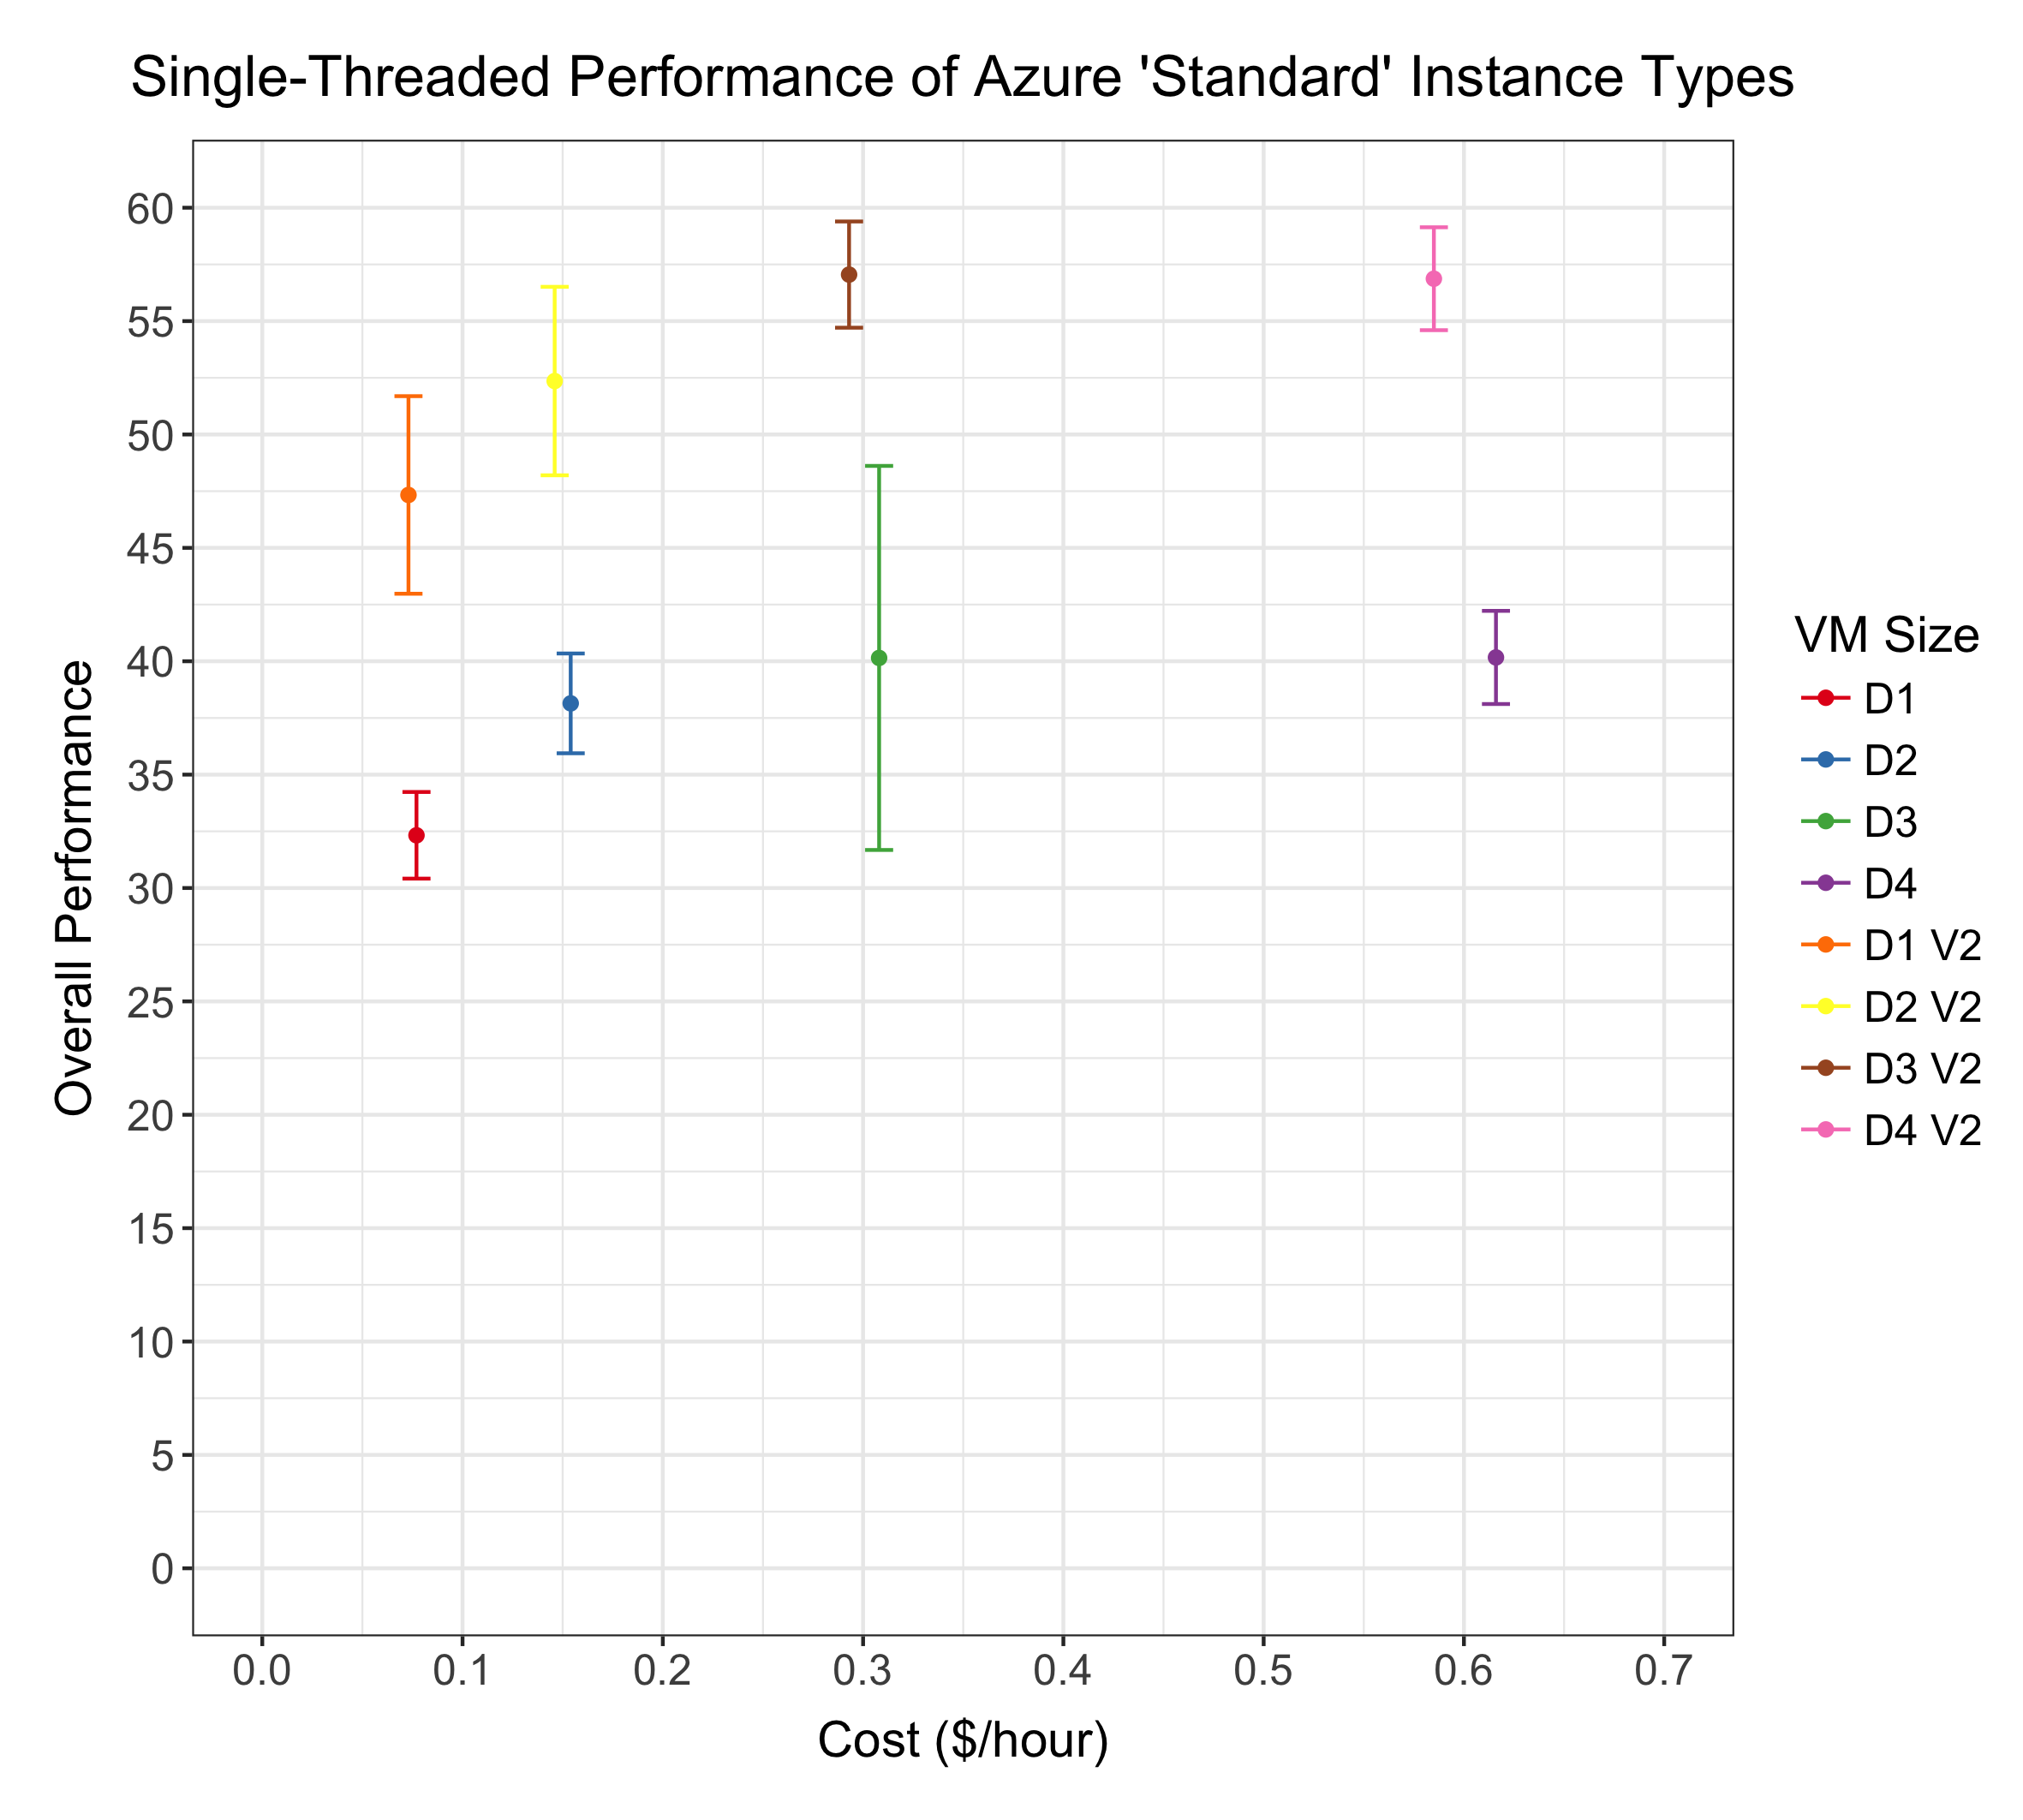
\includegraphics[width=\linewidth]{\graphs/data_azure_single_thread.png}
  \caption{Azure single-threaded average performance results with variance}
  \label{fig:threadvariability}
\end{figure}
% =====================

The different VM types of a particular series appear to have very similar single-threaded performance across most tests. This is most likely due to the different instance tiers within a series being provisioned from the same hardware, with virtualisation techniques in place over the top. The maximum clock speed of the CPUs would be the same, resulting in near identical single-threaded performance. However, the `sunflow' test does appear to improve from one instance to the next, apart from the largest instance type, the D4. This is due to the nature of the test, whereby one bundle of 4 threads is used per hardware thread. When running in single-threaded mode, the test is still creating 4 threads which see increased performance as the number of hardware threads increases, up to 4 cores \cite{shiv2009specjvm2008}. The D4 instance has 8 cores, and so would not perform more optimally unless a second bundle was introduced. This has a negative impact on the results, and so overall figures have also been calculated with the sunflow test removed. When comparing the D-series to the Dv2-series as a whole, there is a substantial increase in performance across all tests. This is a direct result of the improved newer CPUs within the Dv2-series, and equates to a near 40\% performance increase. However, one outlier arose during the testing process on one of the Standard\_D3 instance types. The benchmark results were significantly greater, by approximately 40\%, across all tests than other instances within the same tier and series (figure \ref{fig:threadvariability}). This single instance of testing in fact showed results that are very similar with instance types within the Dv2-series. Without further testing taking place it is difficult to identify the underlying cause of this result.

% % Graph of single threaded performance on azure
% % =====================
% \begin{figure}[ht]
%   \centering
%   \includegraphics[width=0.8\linewidth]{singlethread.png}
%   \caption{Azure single threaded performance on both D and Dv2 series}
%   \label{fig:threadchart}
% \end{figure}
% % =====================

Another avenue of extended testing took the form of measuring performance over time. The intention of which is to see if the performance can improve over time when a freshly instantiated instance performs poorly initially, or whether there will be continually lesser performance. However, rather than running the entire benchmark after provisioning an instance, one test was used to give an indication of how well the VM performed. The compression test out of the SPECjvm2008 benchmark suite was chosen, as it represents the power of the underlying systems well in the tests so far. The test itself also scales near linearly with the number of threads \cite{shiv2009specjvm2008}, which should provide better performance estimates on multi-core machines. To measure the performance of instances over time, this single `compress' test was run on 10 separate Standard\_D1\_v2 instances a total of 6 times, with a 10 minute break between runs. The results can be seen in table \ref{tab:timeazure}, where the penultimate 2 columns indicate the max difference between the first iteration and all subsequent iterations, and the difference from the average for the last column.

% % Performance over time results Table
% % =====================
\begin{table*}[!h]
  \caption{Compression test ran every ten minutes on 10 different instances}
  \label{tab:timeazure}
  \begin{adjustbox}{width=\linewidth,center}
    \small
      % \csvautotabul\end{adjustbox}arcustom[respect all]{\data/time_results.csv}
      \begin{tabular}{|R{\rcolfive}|R{\rcolfive}|R{\rcolfive}|R{\rcolfive}|R{\rcolfive}|R{\rcolfive}|R{\rcolfive}|R{\rcolfive}|R{\rcolfive}|R{\rcolfive}|R{\rcolfive}|R{\rcolfive}|}
        \hline
Instance & Iteration 1 & Iteration 2 & Iteration 3 & Iteration 4 & Iteration 5 & Iteration 6 & Average & max decrease & max increase & from average \\ \hline
1 & 51.19 & 51.86 & 51.64 & 50.42 & 51.95 & 51.62 & 51.45 & -0.77 & 0.76 & 0.26 \\
2 & 51.97 & 50.48 & 51.72 & 52.15 & 51.01 & 51.39 & 51.45 & -1.49 & 0.18 & 0.52 \\
3 & 49.4 & 50.24 & 49.88 & 50.03 & 49.75 & 50.27 & 49.93 & 0 & 0.87 & 0.53 \\
4 & 47.8 & 48.37 & 47.05 & 47.58 & 47.43 & 48.81 & 47.84 & -0.75 & 1.01 & 0.04 \\
5 & 48.77 & 51.37 & 50.29 & 51.08 & 50.35 & 50.35 & 50.37 & 0 & 2.6 & 1.6 \\
6 & 49.7 & 48.93 & 48.85 & 49.85 & 48.48 & 48.81 & 49.1 & -1.22 & 0.15 & 0.6 \\
7 & 51.71 & 51.27 & 51.56 & 51.23 & 50.42 & 50.87 & 51.18 & -1.29 & 0 & 0.53 \\
8 & 49.64 & 50.33 & 52.05 & 50.65 & 51.67 & 50.58 & 50.82 & 0 & 2.41 & 1.18 \\
9 & 47.68 & 49.16 & 49.55 & 49.15 & 49.75 & 48.94 & 49.04 & 0 & 2.07 & 1.36 \\
10 & 50.26 & 49.97 & 48.74 & 49.07 & 49.68 & 49.2 & 49.49 & -1.52 & 0 & 0.77 \\
 &  &  &  &  &  &  & 50.07 & -0.7 & 1.01 & 0.74 \\ \hline
      \end{tabular}
    \end{adjustbox}
\end{table*}
% % =====================

The output of the compression test is very similar across the board for this set of tests, with the results deviating by only 6\% lower and 4\% higher performance than the overall average. Some of the instances remained relatively consistent across all 6 iterations, such as instance numbers 3 and 7, with a maximum change in result between runs at 0.84 and 0.81 respectively. Others performed more erratically, such as instance 5, where the compression result increases by 2.60 from the first iteration to the second. Instance 4 performed particularly poorly when compared to the others, with the lowest score seen in the third iteration, and no scores above 48.81. Half of the instances did not produce results that low, and the lowest score of another three were not far below this value. The higher performing instances, 1, 2, and 7, all scored above 50.42, with an average score greater than 51.18.

The intention for this set of testing however is to evaluate how the first test iteration performs in relation to the rest of the results. In 40\% of cases, the initial test iteration was the lowest score seen, with the performance increasing by more than 2.00 points in three of them. However, in two of the instance results, the initial test run result was the highest seen over the time period, with a decrease in performance from this result by as much as 1.52.

The difference from the initial result to the average score for the VM across the results ranged from 0.04, where the initial result gave a good indication to the performance of the instance, to 1.60 where the average was greater than the initial result would have indicated. These differences from the initial result show that it is hard to judge an instance from an initial reading; in some cases this can work well, but others it will not. The variability from one instance to the next would make this method impractical to measure a VMs performance before making use of it. To refine this approach, the initial test could be run for a longer duration in an attempt to get a better representation of the instances performance. Different VM types may also perform less or more variably over time, and so a higher instance tier may produce more useful results.

%% CONCLUSION
%% =========================================================================================================================

\section{Conclusions}

Throughout this research, the intent has been to create a benchmarking tool to collect performance information of cloud infrastructure, which can in turn be used to make superior scheduling decisions. The tool has been designed to permit the direct comparison of compute performance from one virtual machine to another, irrespective of the service provider. At the time of writing, the presented system may only support the SPECjvm2008 test suite, however the end goal is for the tool to act as a harness for other benchmarking software. Whilst others, \cite{li2010cloudcmp}, \cite{chhetri2013smart}, perform similar experiments to those covered here, we aim to provide this tool as an available open-source system for others to use~\footnote{https://github.com/NewcastleComputingScience/cloud-performance}. The tool has been used to measure a wide variety of instance type offerings from two different cloud service providers, where it is observed that an increase in cost does not always reflect in higher compute performance.


%
% ---- Bibliography ----
%
\bibliographystyle{entcs}
\bibliography{IEEEabrv,research}
% \bibliography{splncs03,research}
\appendix
% \begin{appendices}
  % \section
  % \renewcommand{\thesection}{\appendixname~\Alph{section}}
  \section{VM Instance Specifications}
  % % Performance over time results Table
  % % =====================
  \begin{table*}[!h]
    \caption{Specifications of Azure instance types}
    \label{tab:azure:specs}
      \begin{adjustbox}{width=0.6\linewidth,center}
      \small
        % \csvautotabularcustom[respect all]{\data/data_azure_specs.csv}
        \begin{tabular}{|L{0.1\linewidth}|L{\lcollengthlarge}|R{\lcollengthlarge}|R{0.08\linewidth}|R{0.08\linewidth}|}
          \hline
VM Type & VM Size & Cores & Memory GB & Cost \$/hour \\ \hline
basic & a1 & 1.00 & 1.75 & 0.044 \\
basic & a2 & 2.00 & 3.50 & 0.088 \\
basic & a3 & 4.00 & 7.00 & 0.176 \\
basic & a4 & 8.00 & 14.00 & 0.352 \\
standard & d1 & 1.00 & 3.50 & 0.077 \\
standard & d2 & 2.00 & 7.00 & 0.154 \\
standard & d3 & 4.00 & 14.00 & 0.308 \\
standard & d4 & 8.00 & 28.00 & 0.616 \\
standard & d11 & 2.00 & 14.00 & 0.195 \\
standard & d12 & 4.00 & 28.00 & 0.390 \\
standard & d13 & 8.00 & 56.00 & 0.780 \\
standard & d1 v2 & 1.00 & 3.50 & 0.073 \\
standard & d2 v2 & 2.00 & 7.00 & 0.146 \\
standard & d3 v2 & 4.00 & 14.00 & 0.293 \\
standard & d4 v2 & 8.00 & 28.00 & 0.585 \\
standard & d11 v2 & 2.00 & 14.00 & 0.185 \\
standard & d12 v2 & 4.00 & 28.00 & 0.371 \\
standard & d13 v2 & 8.00 & 56.00 & 0.741 \\ \hline
        \end{tabular}
      \end{adjustbox}
  \end{table*}
  % % =====================

  % % Performance over time results Table
  % % =====================
  \begin{table*}[!h]
    \caption{Specifications of EC2 instance types}
    \label{tab:aws:specs}
      \begin{adjustbox}{width=0.6\linewidth,center}
        \small
        % \csvautotabularcustom[respect all]{\data/data_aws_specs.csv}
        \begin{tabular}{|L{0.1\linewidth}|L{0.08\linewidth}|R{\lcollengthlarge}|R{0.08\linewidth}|R{0.08\linewidth}|}
          \hline
VM Type & VM Size & Cores & Memory GB & Cost \$/hour \\ \hline
t2 & micro & 1.00 & 1.00 & 0.014 \\
t2 & small & 1.00 & 2.00 & 0.028 \\
t2 & med & 2.00 & 4.00 & 0.056 \\
t2 & large & 2.00 & 8.00 & 0.112 \\
m4 & large & 2.00 & 8.00 & 0.132 \\
m4 & xlarge & 4.00 & 16.00 & 0.264 \\
m4 & 2xlarge & 8.00 & 32.00 & 0.528 \\
c4 & large & 2.00 & 3.75 & 0.119 \\
c4 & xlarge & 4.00 & 7.50 & 0.238 \\
c4 & 2xlarge & 8.00 & 15.00 & 0.477 \\ \hline
        \end{tabular}
      \end{adjustbox}
  \end{table*}
  % % =====================
% \end{appendices}



\end{document}
